\documentclass[a4paper,12pt]{scrbook}

\usepackage{fontspec}
\usepackage{polyglossia}
%\setdefaultlanguage[spelling=new,latesthyphen=true,babelshorthands=true]{german}
\setdefaultlanguage[spelling=new,latesthyphen=true]{german}

\setmainfont[Mapping=tex-text,Numbers=OldStyle,Ligatures=Rare]{Linux Libertine O}
\setsansfont{Linux Biolinum O}

\usepackage{csquotes}
\usepackage{hyperref,amsmath,amsfonts,amssymb,bbm,enumitem}
\usepackage[thmmarks,amsmath,thref,hyperref]{ntheorem}
\usepackage{cleveref}

\def\filename{alggeo.sublinks}
\newcommand{\readfromfile}[1]{\input{#1}}
% coole Datei mit Formaten einlesen und dann neue erstellen:
% Existenz überprüfen:
\newread\foo
\immediate\openin\foo=\filename\relax
\ifeof\foo\relax%überprüfen ob schon vorhanden
\else\readfromfile\filename\relax\fi
\immediate\closein\foo
\newwrite\blah
\immediate\openout\blah=\filename\relax
%% und am Ende wieder zu machen:
\AtEndDocument{\immediate\write\blah{\string\endinput}\relax \immediate\closeout\blah}

\usepackage{tikz}
\usetikzlibrary{matrix,arrows,calc}

\deffootnote[1em]{1em}{1em}{\textsuperscript{\thefootnotemark}\ }
\setlength{\parindent}{0pt}
\setlength{\parskip}{3pt}

\begingroup
\catcode`\#=12
\gdef\hashchar{#}%
\endgroup

\newtheorem{thmcnt}{Dummy}[section]
\newcommand{\definetheorem}[3]{
  \np %nummerierte Variante
  \newtheorem{#1}[#3]{#2}
  \nnp %unnummerierte Variante
  \newtheorem{n#1}[#3]{#2}
  \BeforeBeginEnvironment{n#1}{\addtocounter{thmcnt}{-1}}%ausgleich, weil er trotzdem weiterzählt...
  \crefformat{#1}{##2#2~##1##3}
  \BeforeBeginEnvironment{#1}{\makeatletter%
     \addtocounter{thmcnt}{1}% noch nicht passiert
     \edef\labelcode{ctr@#1@\roman{chapter}@\roman{section}@\arabic{thmcnt}}\relax%
     % formatierungszeugs wird in datei geschrieben, so dass es beim nächsten mal rechtzeitig eingelesen und verwendet werden kann...
     \immediate\write\blah{\string\crefname{\labelcode}{#2\noexpand~\thethmcnt}{}}\relax%
    % jetzt noch die Formatierungsinformationen mit rein...
    \immediate\write\blah{\string\crefformat{\labelcode}{\string##2#2\noexpand~\thethmcnt\noexpand~\hashchar1\hashchar3}}%
      % neuer Befehl: Label setzt richtigen label für Aufzählungen in Umgebungen
      \edef\Label##1{\noexpand\label[\labelcode]{##1}}%
      \addtocounter{thmcnt}{-1} % schnell wieder zurück :)
  \makeatother}%
}

% coole gabi-style umgebungen:
%\makeatletter
%\newtheoremstyle{keinenummern}{\item[\theorem@headerfont]{\sc##1}}{\item[\theorem@headerfont](##3)}
%\makeatother
% Format ohne Nummern
\newcommand{\nnp}{%
  \theoremstyle{nonumberplain}%
  %\theoremstyle{keinenummern}
  \theorempreskipamount0pt plus 2pt\relax%
  \theorempostskipamount0pt plus 2pt\relax%
  \theoremheaderfont{\hspace*{-2.5em}\sc}%
  \theorembodyfont{\normalfont}%
  \theoremseparator{:}%
  \theoremindent3em\relax%
}
%Format mit Nummern
\newcommand{\np}{%
  \theoremstyle{plain}
  \theorempreskipamount0pt plus 2pt\relax
  \theorempostskipamount0pt plus 2pt\relax
  \theoremheaderfont{\hspace*{-2.5em}\sc}%
  \theorembodyfont{\normalfont}%
  \theoremseparator{:}%
  \theoremindent3em\relax%
  \theoremnumbering{arabic}%
}
\nnp % ab hier ohne Nummern
\theoremsymbol{}%
\newtheorem{ziel}{Ziel}
\newtheorem{motivation}{Motivation}
\newtheorem{zeige}{Zeige}
\newtheorem{q}{Frage}
%Beweise:
\theoremsymbol{\ensuremath{\Box}}
\newtheorem{proof}{Beweis}
% ab hier mit nummer, n### ohne...
\theoremsymbol{}%
\definetheorem{dfn}{Definition}{thmcnt}
\definetheorem{bsp}{Beispiel}{thmcnt}
\definetheorem{lem}{Lemma}{thmcnt}
\definetheorem{prop}{Proposition}{thmcnt}
\definetheorem{kor}{Korollar}{thmcnt}
\definetheorem{bem}{Bemerkung}{thmcnt}
\definetheorem{erinnerung}{Erinnerung}{thmcnt}
\definetheorem{db}{Definition/Bemerkung}{thmcnt}
\definetheorem{de}{Definition/Erinnerung}{thmcnt}
\definetheorem{dl}{Definition/Lemma}{thmcnt}
\definetheorem{eb}{Erinnerung/Bemerkung}{thmcnt}
% Sätze separat...
\np
\theorembodyfont{\normalfont\it}
\theoremheaderfont{\hspace*{-2.5em}\bf}
\crefformat{satz}{#2Satz~#1#3}
\newtheorem{satz}{Satz}
%\definetheorem{satz}{Satz}{satzcnt}

%Format für Querverweise auf Formeln:
\crefformat{equation}{#2(#1)#3}
\crefformat{chapter}{#2Kapitel~#1#3}

% Warnungen :)
\usepackage{manfnt,environ}
\NewEnviron{w}{\begin{center}\begin{tikzpicture}%
\node[right,text width=0.85\textwidth,rounded corners,fill=orange,inner sep=1ex]{%
  \hbox{\hspace{1em}\makebox[\width][t]{\raisebox{1.3ex}{\lhdbend}}\hspace{2em}%
  \begin{minipage}[c]{.85\textwidth}\smallskip\BODY\medskip\end{minipage}%
}};\end{tikzpicture}\end{center}\par}

\usepackage{textcomp}
\newcommand{\sect}[1]{\begin{tikzpicture}%
\node[right,text width=\textwidth,rounded corners,fill=blue!15,inner sep=5pt]{%
  \hbox{%
  \begin{minipage}[c]{.96\textwidth}\section{#1}\end{minipage}%
  \hfill\makebox[\width][t]{\raisebox{-5pt}{\raisebox{4pt}{\textleaf}}}%
}};\end{tikzpicture}\nopagebreak[4]\markright{\thesection. #1}}

\DeclareMathAlphabet{\mathpzc}{OT1}{pzc}{m}{it}

\def\C{\mathbb{C}}
\def\A{\mathbb{A}}
\def\V{\mathfrak{V}}
\def\VV{\mathcal{V}}
\def\I{\mathfrak{I}}
\def\O{\mathcal{O}}
\def\P{\mathbb{P}}
\newcommand{\D}{\mathfrak{D}}
\newcommand{\DD}{\mathcal{D}} % Dehomogenierung
\renewcommand{\H}{\mathcal{H}} % Homogenisierung
\def\B{\mathcal{B}}
\def\S{\mathcal{S}}
\newcommand{\J}{\mathcal{J}}
\newcommand{\AffVar}{\mathpzc{AffVar}}
\newcommand{\RedAlg}{\mathpzc{RedAlg}}
\newcommand{\Grp}{\mathpzc{Grp}}
\newcommand{\Cat}{\mathpzc{Cat}}
\newcommand{\Set}{\mathpzc{Set}}
\newcommand{\Top}{\mathpzc{Top}}
\newcommand{\Ob}{\mathpzc{Ob}}
\newcommand{\Ar}{\mathpzc{Ar}}
\newcommand{\F}{\mathcal{F}}
\newcommand{\FF}{\mathbb{F}}
\def\G{\mathcal{G}}
\renewcommand{\L}{\mathcal{L}}
\def\T{\mathcal{T}}
\def\M{\mathcal{M}}
\newcommand{\Hom}{\mathrm{Hom}}
\newcommand{\Rat}{\mathrm{Rat}}
\newcommand{\Mor}{\mathrm{Mor}}
\newcommand{\Kern}{\operatorname{Kern}}
\newcommand{\Spec}{\operatorname{Spec}}
\newcommand{\Abb}{\mathrm{Abb}}
\newcommand{\Func}{\mathrm{Func}}
\newcommand{\Nat}{\mathrm{Nat}}
\newcommand{\id}{\mathrm{id}}
\newcommand{\dom}{\operatorname{dom}}
\newcommand{\Def}{\operatorname{Def}}
\newcommand{\cod}{\operatorname{cod}}
\newcommand{\Cone}{\mathrm{Cone}}
\newcommand{\op}{\mathrm{op}}
\newcommand{\Eq}{\mathrm{Eq}}
\renewcommand{\phi}{\varphi}
\newcommand{\ep}{\varepsilon}
\newcommand{\da}{:=}
\newcommand{\leer}{\ensuremath{\varnothing}}
\newcommand{\Quot}{\mathrm{Quot}}
\newcommand{\GL}{\mathrm{GL}}
\newcommand{\card}[1]{|#1|}
\newcommand{\restrict}[1]{|_{#1}}

\newcommand{\set}[1]{\ensuremath{\mathbb{#1}}}
\newcommand{\Q}{\set{Q}}
\newcommand{\N}{\set{N}}
\newcommand{\R}{\set{R}}
\newcommand{\Z}{\set{Z}}

%coole tikzpfeile :)
\newcommand{\smapsto}{\mapsto}
\newcommand{\ra}{\raisebox{-1pt}{\tikz{\draw[thin,shorten >=3pt, ->] (0,0) node{\hspace*{-2pt}} -- node{} (1,0);}}\penalty1000\relax}
\renewcommand{\mapsto}{\raisebox{-1pt}{\tikz{\draw[thin,shorten >=3pt, |->] (0,0) node{\hspace*{0pt}} -- node{} (1,0);}}\penalty1000\relax}
\newcommand{\inj}{\raisebox{-1pt}{\tikz{\draw[thin,shorten >=3pt, right hook->] (0,0) node{\hspace*{0pt}} -- node{} (1,0);}}\penalty1000\relax}
\newcommand{\surj}{\raisebox{-1pt}{\tikz{\draw[thin,shorten >=3pt, ->>] (0,0) node{\hspace*{0pt}} -- node{} (1,0);}}\penalty1000\relax}
% ``punktierte'' Pfeile...
\newcommand{\ppf}{\raisebox{-1pt}{\tikz{\draw[densely dashed,thin,shorten >=3pt, ->] (0,0) node{\hspace*{-2pt}} -- node{} (1,0);}}\penalty1000\relax}

\newcommand{\dach}{\widehat}
\newcommand{\oldbar}[1]{\bar{#1}}
\def\Bar#1{\ensuremath\overline{#1}}

\newcommand{\Quotient}[2]{
  \raisebox{0.7ex}{\ensuremath{#1}}
  \ensuremath{\mkern-3mu}\big/\ensuremath{\mkern-3mu}
  \raisebox{-0.6ex}{\ensuremath{#2}}}

%Listenformate:
\setenumerate[1]{leftmargin=*,labelindent=\parindent,label=(\alph*)}
\setenumerate[2]{leftmargin=*,labelindent=\parindent,label=(\roman*)}
%seperate listen im Beweise
\newlist{prooflist}{enumerate}{2}
\setlist[prooflist]{leftmargin=*,labelindent=\parindent,label=(\arabic*)}
\setlist[prooflist,2]{label=(\roman*)}

%Polynomringe
\newcommand{\polyx}[1][n]{\ensuremath%
  [X_{1},\dotsc,X_{#1}]}
% im projektiven wollen wir mit 0 anfangen; mehrere optionale Argumente sind leider nicht ohne weiteres möglich...
\newcommand{\ppolyx}[1][n]{\ensuremath%
  [X_{0},\dotsc,X_{#1}]}

% sectionformat:
\renewcommand{\thesection}{\arabic{section}}
\renewcommand{\thechapter}{\textsc{\roman{chapter}}}

\author{JProf. Dr. Gabriela Weitze-Schmithüsen}
\publishers{\small Jonathan Zachhuber, Jens Babutzka und Michael Fütterer \\ Karlsruher Institut für Technologie}
\subject{Skript zur Vorlesung}
\title{Algebraische Geometrie I}
\titlehead{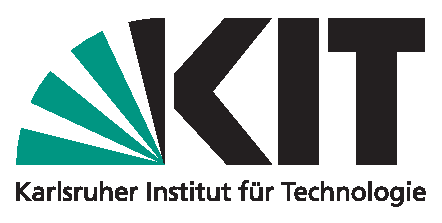
\includegraphics[scale=0.6]{kitlogo}}
\date{Wintersemester 2010/2011}

\begin{document}

\maketitle
\tableofcontents

% 18.10.10
%\setcounter{chapter}{-1}
\chapter*{Motivation}

\begin{ziel}
Untersuche Nullstellenmengen von Polynomen: Für eine Menge von Polynomen
\[p_{1},\dotsc,p_{r}\in k\polyx\]
über einem Körper $k$ möchte man die Menge der Nullstellen
\[\{x=(x_{1},\dotsc,x_{n})\mid p_{i}(x)=0\text{ für alle }i\}\]
analysieren.
\end{ziel}

\begin{nbsp}
\begin{enumerate}
\item Betrachte $ax^{2}+by^{2}=1\iff x^{2}+y^{2}-1=0$ über $k=\R$. Das liefert eine Ellipse, für $a=b=1$ einen Kreis.
%Bild...
\item Betrachte $x^{2}+y^{2}=z^{2}$.
%Bild...
\item Betrachte (b) mit $x=1$: Dann ist $1+y^{2}=z^{2}\iff 1=z^{2}-y^{2}$, also eine Hyperbel.
%Bild
\item Bei linearen Gleichungen sehen wir mit Hilfe der linearen Algebra, das wir affine Unterräume erhalten.
\item Die Lösungsmengen sind abhängig vom Körper, z.B. sehen wir für $k=\Z/3\Z$ hat das Polynom $X^{3}-X$ als Lösungsmenge ganz $k$.
\end{enumerate}
\end{nbsp}

% Rest kommt noch ;)

\chapter{Die Kategorie der affinen Varietäten}\label{kap1}
\sect{Affine Varietäten und Verschwindungsideale}

Sei $k$ stets ein Körper.

\begin{dfn}
$V\subseteq k^{n}$ heißt \emph{affine Varietät}, wenn
$\F\subseteq k\polyx$
mit \[V=\V(\F):=\{x=(x_{1},\dotsc,x_{n})\in k^{n}\mid f(x)=0\;\forall f\in\F\}\] existiert.
\end{dfn}

\begin{bsp}\label{bsp1.2}
\begin{enumerate}
\item $k^{n}=\V(\{0\})$
\item $\leer=\V(\{1\})$
\end{enumerate}
\end{bsp}

\begin{q}Wie eindeutig ist das $\F$? Zum Beispiel liefern Produkte und Summen von Polynomen keine neuen Nullstellen.
\end{q}

\begin{nbsp}\begin{enumerate}
\item $\V(x^{2}+y^{2}+z^{2}-1) \supsetneq \V(x^{2}+y^{2}+z^{2}-1, z-\frac{1}{2})$
\item $\V(x^{2}+y^{2}+z^{2}-1, z-\frac{1}{2}) = \V(x^{2}+y^{2}+z^{2}-1, z-\frac{1}{2}, x^{2}+y^{2}+z^{2}-1 + z-\frac{1}{2}).$
\end{enumerate}\end{nbsp}


\begin{bem}\label{1.1.3} Seien $\F_{1},\F_{2}\subseteq k\polyx$. Dann gilt:
\begin{enumerate}
\item\Label{1.1.3a} $\F_{1}\subseteq\F_{2}\implies \V(\F_{1})\supseteq \V(\F_{2})$
\item\Label{1.1.3b} Sei $(\F)$ das von $\F$ erzeugte Ideal. Dann gilt: $\V(\F) = \V((\F))$.
\item\Label{1.1.3c} Sei
\[\sqrt{(\F)}:=\{p\in k\polyx\mid\exists\, d\geq 1\text{ mit }p^{d}\in(\F)\}\]
das \emph{Radikalideal} von $(\F)$ ($\sqrt{(\F)}$ ist Ideal!). Dann gilt: $\V(\sqrt{(\F)})=\V(\F)$.
\item\Label{1.1.3d} Zu jeder affinen Varietät $V\subseteq k^{n}$ gibt es endlich viele Polynome $f_{1},\dotsc,f_{r}$ mit \[V=\V(\{f_{1},\dotsc,f_{r}\})=:\V(f_{1},\dotsc,f_{r}).\]
\end{enumerate}
\end{bem}

\begin{proof}\mbox{} %damit der link nicht überspring...
\ref{1.1.3a} und \ref{1.1.3b} folgen direkt aus der Definition.
\begin{enumerate}%\addtocounter{enumi}{2}
\item[\ref{1.1.3c}] Offenbar ist $\sqrt{(\F)}\supseteq(\F)$, also gilt nach \ref{1.1.3a} und \ref{1.1.3b}: 
\[\V(\sqrt{(\F)})\subseteq \V((\F))=\V(\F).\]

Für die andere Richtung: Sei $x=(x_{1},\dotsc,x_{n})\in \V(\F)$ und $f\in\sqrt{(\F)}$. Nach Definition existiert $d\in\N$, so dass $f^{d}\in(\F)$. Also gilt $f^{d}(x)=0$ und damit $f(x)=0$, demnach ist $x\in \V(\sqrt{(\F)})$.
\item[\ref{1.1.3d}] Nach \ref{1.1.3b} gilt $\V(\F)=\V((\F))$ und nach Hilberts Basissatz wird $(\F)$ von endlich vielen Elementen erzeugt.
\end{enumerate}
\end{proof}

\begin{db}
Sei $V\subseteq k^{n}$. Wir nennen
\[\I(V):=\{f\in k\polyx\mid f(x)=0\;\forall x\in V\}\]
das \emph{Verschwindungsideal von $V$}. Es ist ein Ideal.
\end{db}

\begin{bem}\label{1.1.5} Es gilt:
\begin{enumerate}
\item\Label{1.1.5a} Seien $V_{1},V_{2}\subseteq k^{n}$ mit $V_{1}\subseteq V_{2}$. Dann ist $\I(V_{1})\supseteq \I(V_{2})$.
\item\Label{1.1.5b} Sei $V\subseteq k^{n}$. Dann ist $\I(V)$ ein Radikalideal.
\item\Label{1.1.5c} Sei $V$ eine affine Varietät. Dann gilt $V=\V(\I(V))$.

Es gilt sogar: $\I(V)$ ist das größte Ideal mit dieser Eigenschaft, d.h. für $J\subseteq k\polyx$ mit $\V(J)=V$ folgt schon $J\subseteq \I(V)$.
\item\Label{1.1.5d} Seien $V_{1},V_{2}$ affine Varietäten. Dann gilt:
\[V_{1}=V_{2}\iff \I(V_{1})=\I(V_{2})\text{ und } V_{1}\subseteq V_{2}\iff \I(V_{1})\supseteq \I(V_{2}).\]
\end{enumerate}
\end{bem}

\begin{proof} Die Aussagen \ref{1.1.5a} und \ref{1.1.5b} folgen sofort aus der Definition.
\begin{enumerate}
\item[\ref{1.1.5c}] Sei zuerst $x\in V$. Dann gilt für alle $f\in \I(V)$: $f(x)=0$, also gilt $x\in \V(\I(V))$.

Sei nun $V$ eine affine Varietät. Dann gilt $V=\V(\F)$ für eine geeignete Menge $\F$. Es gilt $\F\subseteq \I(V)$, also ist
\[V=\V(\F)\supseteq \V(\I(V)).\]

Der Rest der Behauptung folgt aus der Definition des Verschwindungsideals.
\item[\ref{1.1.5d}] Die eine Richtung ist klar, bzw. folgt aus \ref{1.1.5a}. Für die andere Richtung überlegt man sich, dass nach \ref{1.1.5c} $V_{1}=\V(\I(V_{1}))=\V(\I(V_{2}))=V_{2}$ gilt.  Die Aussage für die Inklusionen folgt analog.
\end{enumerate}
\end{proof}

\begin{q}
Wir haben gesehen, dass die Zuordnung
\[V\mapsto \I(V)\]
injektiv ist. Ist sie auch surjektiv?
\end{q}

\sect{Zariski-Topologie}

\begin{db}\label{1.2.1}Sei $n\in\N$. Die affinen Varietäten im $k^{n}$ bilden die abgeschlossenen Mengen einer Topologie auf dem $k^{n}$. Diese heißt \emph{Zariski-Topologie}.\end{db}
\begin{proof}\begin{prooflist}
\item $\leer$ und $k^{n}$ sind affine Varietäten nach \cref{bsp1.2}.
\item Seien $V_{1},V_{2}$ affine Varietäten, d.h. $V_{1}=\V(I_{1})$ und $V_{2}=\V(I_{2})$, wobei $I_{1},I_{2}$ Ideale in $k\polyx$ sind. Dann gilt:
\[V_{1}\cap V_{2}=\V(I_{1}\cup I_{2}) = \V(I_{1}+I_{2}).\]
Das gleiche Argument funktioniert für beliebige Familien $V_{\lambda}$ mit $\lambda\in\Lambda$ und $\Lambda$ Indexmenge, d.h. $\displaystyle\bigcap_{\lambda\in\Lambda}V_{\lambda}$ ist wieder eine affine Varietät.
% 20.10.2010
\item Seien $V_{1},V_{2}$ affine Varietäten mit $I_{1}=\I(V_{1})$ und $I_{2}=\I(V_{2})$.
\begin{zeige} $\V(I_{1}\cdot I_{2})\subseteq V_{1}\cup V_{2}\subseteq \V(I_{1}\cap I_{2})\subseteq \V(I_{1}\cdot I_{2})$.
\begin{prooflist}
\item $V_{1}\cup V_{2}\subseteq \V(I_{1}\cap I_{2})$ ist nach Definition klar.
\item Sei $x\in \V(I_{1}\cdot I_{2})$. Angenommen $x\notin V_{1}$. Dann existiert $g\in I_{1}$ mit $g(x)\neq 0$. Sei $f\in I_{2}$. Dann ist $f\cdot g\in I_{1}\cdot I_{2}$, also ist $f\cdot g(x) = f(x)\cdot g(x) = 0$ und da $g(x)\neq 0$ ist $f(x)=0$, also $x\in \V(I_{2})=V_{2}$.
\end{prooflist}\end{zeige}
\end{prooflist}\end{proof}

\begin{dfn}\label{1.2.2}
Schreibe $\A^{n}(k)$ für $k^{n}$ mit der Zariski-Topologie.
\end{dfn}

\begin{bem}\label{1.2.3}
Sei $M\subseteq\A^{n}(k)$. Der Abschluss $\Bar{M}$ von $M$ bezüglich der Zariski-Topologie ist $\Bar{M}=\V(\I(M))$.
\end{bem}
\begin{proof}
$\Bar{M}\subseteq \V(\I(M))$ folgt sofort aus der Definition.

Für die andere Inklusion überlegt man sich: Sei $M\subseteq\V(J)$ eine abgeschlossene Obermenge von $M$. Dann ist $\I(M)\supseteq\I(\V(J))$ und damit
\[\V(\I(M))\subseteq\V(\I(\V(J)))=\V(J).\]
\end{proof}

\begin{bsp}\label{1.2.4}
Sei $n=1$. Dann gilt: $X\subseteq\A^{1}(k)$ ist genau dann abgeschlossen, wenn $X$ eine endliche Teilmenge oder ganz $\A^{1}(k)$ ist.
\end{bsp}

\begin{w}\enquote{Kleine Umgebungen} sind riesig groß!\end{w}

\begin{bem}\label{1.2.5}
\begin{enumerate}
\item\Label{1.2.5a} Wenn $k$ endlich ist, entspricht die Zariski-Topologie auf $\A^{1}(k)$ der diskreten Topologie.
\item\Label{1.2.5b} Wenn $k$ unendlich ist, ist die Zariski-Topologie nicht hausdorffsch.
\end{enumerate}\end{bem}
\begin{proof}\begin{enumerate}
\item[\ref{1.2.5a}] Punkte sind abgeschlossen, denn sei $x=(x_{1},\dotsc,x_{k})\in k^{n}$, dann ist
\[{x}=\V(X_{1}-x_{1},\dotsc,X_{n}-x_{n}).\]
Damit sind auch endliche Vereinigungen von Punkten abgeschlossen und somit schon \emph{alle} Teilmengen von $\A^{1}(k)$.
\item[\ref{1.2.5b}] {\sc Erinnerung:} Ein topologischer Raum $X$ heißt hausdorffsch, wenn für alle $x,y\in X$ offene Umgebungen $U_{x}\ni x$ und $U_{y}\ni y$ mit $U_{x}\cap U_{y}=\leer$ existieren.

Für $n=1$ folgt die Behauptung also aus \cref{1.2.4}.

Den Fall $n\geq 2$ führen wir zurück auf den Fall $n=1$:

Seien $x,y\in\A^{n}(k)$, $U_{x},U_{y}$ offene Umgebungen von $x$ bzw. $y$. Wir setzen
\[V_{1}:=\A^{n}(k)\setminus U_{x} = \V(I_{1})\text{ und }V_{2}:=\A^{n}(k)\setminus U_{y}=\V(I_{2})\]
für entsprechende Ideale $I_{1}$ und $I_{2}$. Ohne Einschränkung gebe es Polynome $f\in I_{1}$ und $g\in I_{2}$, in denen $X_{1}$ als Variable vorkommt (sonst

\begin{w}Hilfe!\end{w}

Sei $W:=\V(X_{2},\dotsc,X_{n})$. Dann besteht $V_{1}\cap W$ aus nur endlich vielen Punkten, da diese Nullstellen von $f(X_{1},0,\dotsc,0)$ sein müssen. Gleiches gilt für $V_{2}\cap W$. Also schneiden sich $U_{x}$ und $U_{y}$ sogar schon in $W$.
\end{enumerate}\end{proof}

\begin{de}\label{1.2.6} Seien $X,X_{1},X_{2}$ topologische Räume.
\begin{enumerate}
\item Sei $Y\subseteq X$. Definiere auf $Y$ die \emph{Spurtopologie} durch
\[U\subseteq Y\text{ offen}\: :\Longleftrightarrow\:\exists\;V\subseteq X\text{ offen mit }U=V\cap Y.\]
\item Sei $X\times Y$ das kartesische Produkt (als Mengen) und seien
\begin{align*}p_{1}\colon X_{1}\times X_{2}\rightarrow X_{1},\quad(x_{1},x_{2})\mapsto x_{1},\\p_{2}\colon X_{1}\times X_{2}\rightarrow X_{2},\quad(x_{1},x_{2})\mapsto x_{2},\end{align*}
die zugehörigen Projektionen. Die \emph{Produkttopologie} auf $X_{1}\times X_{2}$ ist die gröbste Topologie (d.h. möglichst wenig offene Mengen), so dass $p_{1}$ und $p_{2}$ stetig sind.

D.h. $U\subseteq X_{1}\times X_{2}$ ist genau dann offen, wenn $U$ beliebige Vereinigung endlicher Schnitte von Urbildern offener Mengen in $X_{1}$ bzw. $X_{2}$ unter $p_{1}$ bzw. $p_{2}$ ist.

\item $X$ heißt \emph{reduzibel}, wenn es abgeschlossene echte Teilmengen $A,B\subsetneq X$ mit $X=A\cup B$ gibt.

\item $X$ heißt \emph{irreduzibel}, wenn $X$ nicht reduzibel ist.

\item Eine maximale irreduzible Teilmenge von $X$ heißt \emph{irreduzible Komponente}.
\end{enumerate}\end{de}

\begin{bsp}\label{1.2.7}
Sei $X$ hausdorffsch und $M\subseteq X$. Dann gilt:
\[M\text{ ist irreduzibel (bzgl. Spurtopologie)}\iff \card{M}\leq 1,\]
d.h. $M$ ist einelementig oder leer.

\emph{Denn}: Liegen $x\neq y$ in $M$, so finden wir (offene) Umgebungen $U_{x}$ und $U_{y}$ mit leerem Schnitt, können also
\[M=(M\setminus U_{x})\cup(M\setminus U_{y})\]
schreiben und sehen so, dass $M$ reduzibel ist. $\leer$ ist nie irreduzibel.
\end{bsp}

\begin{bsp}\label{1.2.8} Sei $k$ ein Körper mit unendlich vielen Elementen.
\begin{enumerate}
\item\Label{1.2.8a} $\A^{1}(k)$ ist irreduzibel, da echte abgeschlossene Teilmengen endlich sind.
\item\label{1.2.8b} $\V(X\cdot Y) = \V(X)\cup\V(Y)$ ist reduzibel mit irreduziblen Komponenten $\V(X)$ und $\V(Y)$.
\end{enumerate}\end{bsp}

\begin{bem}\label{1.2.9}
Sei $V\subseteq\A^{n}(k)$ eine affine Varietät. Dann gilt:
\[V\text{ ist irreduzibel}\iff\I(V)\text{ ist ein Primideal}.\]
\end{bem}
\begin{proof}
Sei zuerst $V$ irreduzibel. Seien $f,g\in k\polyx$ mit $f\cdot g\in\I(V)$. 

Angenommen $f\notin\I(V)$, dann gilt auch $\V(f)\not\supseteq\V(\I(V))=V$.

Andererseits gilt nach \cref{1.2.1}: $\V(f)\cup\V(g)=\V(f\cdot g)\supseteq V$, also
\[V=(V\cap \V(f))\cup(V\cap\V(g)),\]
wobei $V\cap\V(f)$ und $V\cap\V(g)$ in $V$ abgeschlossen sind. Außerdem ist $V\neq V\cap\V(f)$, also gilt, da $V$ irreduzibel ist, $V=V\cap\V(g)$. Daraus folgt $V\subseteq\V(g)$ und damit ist $g\in\I(V)$ und $\I(V)$ ist somit ein Primideal.

Sei nun $\I(V)$ ein Primideal. Seien $V_{1},V_{2}$ Varietäten mit $V=V_{1}\cup V_{2}$ und $I_{1}:=\I(V_{1})$, $I_{2}:=\I(V_{2})$.

Angenommen $V\neq V_{1}$, d.h. $V\supsetneq V_{1}$, dann ist auch $\I(V)\subsetneq\I(V_{1})=I_{1}$.

Andererseits ist $V=V_{1}\cup V_{2}=\V(I_{1}\cdot I_{2})$, also ist $I_{1}\cdot I_{2}\subseteq\I(V)$. Das impliziert aber $I_{2}\subseteq\I(V)$, da $\I(V)$ ein Primideal ist und $I_{1}\not\subseteq\I(V)$. Daher gilt $V_{2}=\V(I_{2})\supseteq\V(\I(V))=V$, also ist schon $V=V_{2}$ und damit ist $V$ irreduzibel.
\end{proof}

\begin{prop}\label{1.2.10} Sei $X$ ein topologischer Raum. Dann ist jede irreduzible Teilmenge in einer irreduziblen Komponente enthalten.\end{prop}
% 25.10.2010
\begin{proof} Verwende das Lemma von Zorn:

{\sc Erinnerung:} Hat in einer halbgeordneten Menge $\M$ jede Kette (d.h. totalgeordnete Teilmenge) eine obere Schranke, dann hat $\M$ mindestens ein maximales Element.

Seien also $X'\subseteq X$ eine irreduzible Teilmenge, $\M:=\{Y\subseteq X\mid Y\text{ irreduzibel, }Y\supseteq X'\}$ und $\{Y_{\lambda}\}_{\lambda\in\Lambda}$ eine Familie aus $\M$, die totalgeordnet ist. Sei $\displaystyle Y:=\bigcup_{\lambda\in\Lambda}Y_{\lambda}$.

{\sc Zeige:} $Y\in\M$, d.h. $Y$ ist irreduzibel.

Wir nehmen an, es gäbe abgeschlossene Mengen $A,B\subsetneq X$, so dass $Y\cap A$ und $Y\cap B$ echte Teilmengen von $Y$ sind, für die $Y=(Y\cap A)\cup(Y\cap B)$ gilt. Insbesondere gilt dann:
\[(X\setminus A)\cap Y\neq\leer\neq (X\setminus B)\cap Y.\]
Folglich existieren ein $\lambda_{1}$ mit $(X\setminus A)\cap Y_{\lambda_{1}}\neq\leer$ und ein $\lambda_{2}$ mit $(X\setminus B)\cap Y_{\lambda_{2}}\neq\leer$. Da die $Y_{\lambda_{i}}$ Teil einer Kette sind, können wir ohne Einschränkung $Y_{\lambda_{1}}\subseteq Y_{\lambda_{2}}$ annehmen. Damit ist aber auch $(X\setminus A)\cap Y_{\lambda_{2}}\neq\leer$ und wir finden eine echte Zerlegung
\[Y_{\lambda_{2}}=(Y_{\lambda_{2}}\cap A)\cup(Y_{\lambda_{2}}\cap B),\]
was im Widerspruch zur Irreduzibilität von $Y_{\lambda_{2}}$ steht. Folglich hat jede Kette eine obere Schranke und nach dem Lemma von Zorn hat $\M$ somit ein maximales Element.
\end{proof}

\begin{satz}\label{satz1} Sei $V$ eine affine Varietät. Dann gilt:
\begin{enumerate}
\item\Label{s1a} $V$ ist eine endliche Vereinigung von irreduziblen affinen Varietäten.
\item\Label{s1b} $V$ hat nur endlich viele irreduzible Komponenten $V_{1},\dotsc,V_{r}$. Insbesondere ist die Zerlegung
\[V=V_{1}\cup\dotsm\cup V_{r}\]
eindeutig.\end{enumerate}\end{satz}
\begin{proof}\begin{enumerate}
\item[\ref{s1a}] Seien 
\begin{align*}&\B:=\{V\subseteq k^{n}\mid V\text{ ist affine Varietät und erfüllt \emph{nicht} \ref{s1a}}\},\\
&\J:=\{\I(V)\subseteq k\polyx\mid V\in\B\}.\end{align*}
Wir nehmen an, $\B$ wäre nicht leer. Dann ist auch $\J$ nicht leer. Da $k\polyx$ noethersch ist, finden wir in $\J$ ein maximales Element $I_{0}=\I(V_{0})$. Damit ist $V_{0}$ ein minimales Element in $\B$. Dann ist $V_{0}$ aber \emph{nicht} irreduzibel, also existieren affine Varietäten $V_{1},V_{2}\subsetneq V$ mit $V=V_{1}\cup V_{2}$. Insbesondere sind diese aber nicht in $\B$, da $V_{0}$ minimal gewählt war, lassen sich also als Vereinigung endlich vieler irreduzibler Varietäten schreiben. Dann geht das aber auch für $V_{0}$ und das ist ein Widerspruch, da $V_{0}\in\B$.
\item[\ref{s1b}] Mit Hilfe von \cref{1.2.10} und dem \ref{s1a}-Teil sehen wir, dass wir \[V=V_{1}\cup\dotsm\cup V_{r}\] schreiben können, wobei die $V_{i}$ irreduzible Komponenten sind. Wir zeigen noch die Eindeutigkeit dieser Zerlegung: Sei $W$ eine irreduzible Komponente von $V$. Wir schreiben
\[W=(W\cap V_{1})\cup\dotsm\cup(W\cap V_{r})\]
und sehen, da $W$ irreduzibel ist, dass es ein $i$ mit $W=W\cap V_{i}$ gibt. Also gilt $W\subseteq V_{i}$ und damit schon $W=V_{i}$, da $W$ als irreduzible \emph{Komponente} eine \emph{maximale} irreduzible Teilmenge von $V$ ist.
\end{enumerate}\end{proof}

\sect{Der Hilbertsche Nullstellensatz}

\begin{motivation}
  Bisher haben wir die Mengen
  \[ \VV_n = \{ V\subseteq k^n \mid V \text{ affine Varietät }\} \quad\text{und}\quad
     \J_n = \{ I\subseteq k\polyx \mid I \text{ Radikalideal }\} \]
  und zwischen ihnen die Abbildungen
  \begin{align*}
    \V\colon& \J_n \ra \VV_n, \quad I\mapsto\V(I)\\
    \I\colon& \VV_n \ra \J_m, \quad V\mapsto\I(V)
  \end{align*}
  betrachtet. Wir haben gesehen, dass $\V\circ\I=\id$ gilt. Gilt auch $\I\circ\V=\id$?
\end{motivation}

\begin{nbsp}
  Wenn $k$ nicht algebraisch abgeschlossen ist, muss das nicht gelten: sei $k=\R$ und $I=(X^2+1)$. Dann ist $\V(I)=\leer$, aber
  $\I(\V(I)) = k\polyx$.
\end{nbsp}

Wir werden sehen, dass $\I\circ\V=\id$ gilt, falls $k$ algebraisch abgeschlossen ist. Die einzige \enquote{Obstruktion} ist,
dass $\V(I)=\leer$ gilt, obwohl $I\neq k\polyx$.

\begin{satz}[Hilbertscher Nullstellensatz]\label{satz2}\label{HNS}
  \begin{enumerate}
  \item\Label{s2a} {\bf Algebraische Form:}\Label{satz2a} Sei $m$ ein maximales Ideal in $k\polyx$. Dann ist $\Quotient{k\polyx}{m}$ eine
    endliche algebraische Körpererweiterung von $k$.
  \item {\bf Schwacher Hilbertscher Nullstellensatz:}\Label{satz2b} Ist $k$ algebraisch abgeschlossen und $I\subsetneq k\polyx$
    ein echtes Ideal, dann ist $\V(I)\neq\leer$.
  \item {\bf Starker Hilbertscher Nullstellensatz:}\Label{satz2c} Ist $k$ algebraisch abgeschlossen und $I\subseteq k\polyx$ ein
    Ideal, dann ist $\I(\V(I))=\sqrt{(I)}$.
  \end{enumerate}
\end{satz}

Die Aussage wird in mehreren Schritten im Rest dieses Abschnitts bewiesen.

Wir bezeichnen $x_1=\Bar{X}_1,\dotsc,x_n=\Bar{X}_n$. Ohne Einschränkung können wir nach einer eventuellen Umsortierung
der Variablen annehmen, dass $x_1,\dotsc,x_k$ algebraisch unabhängig über $k$ sind und $x_{k+1},\dotsc,x_n$ algebraisch über
$k(x_1,\dotsc,x_k)$. Also:
\[ k \subseteq S = k(x_1,\dotsc,x_k) \subseteq L=\Quotient{k\polyx}{m}, \]
dabei ist $k(x_1,\dotsc,x_k)\cong\Quot(k\polyx[k])$ und $L$ ist endlich erzeugt als $S$-Modul.

\begin{lem}\label{1.3.1}
  Seien $R$, $S$, $T$ Ringe mit $R\subseteq S\subseteq T$, sodass gilt:
  \begin{itemize}
  \item $R$ ist noethersch
  \item $T$ ist endlich erzeugt als $R$-Algebra; seien $x_1,\dotsc,x_n$ solche Erzeuger
  \item $T$ ist endlich erzeugt als $S$-Modul; seien $w_1,\dotsc,w_m$ solche Erzeuger
  \end{itemize}
  Dann ist $S$ als $R$-Algebra endlich erzeugt.
\end{lem}
\begin{proof}
  Wir schreiben 
  \[ x_i=\displaystyle\sum_{j=1}^m a_{ij}w_j \text{ mit } a_{ij}\in S, \qquad
     w_iw_j=\displaystyle\sum_{k=1}^m b_{ijk}w_k \text { mit } b_{ijk}\in S. \]
  Sei $S_0$ die $R$-Unteralgebra von $S$, die von allen $a_{ij}$ und $b_{ijk}$ erzeugt wird. Nach dem Hilbertschen Basissatz ist
  $S_0$ ein noetherscher Ring. $T$ wird von den $w_i$ auch als $S_0$-Modul erzeugt und ist noethersch als $S_0$-Modul, da er ein
  endlich erzeugter Modul über einem noetherschen Ring ist. $S$ ist ein $S_0$-Untermodul von $T$. Damit ist $S$ endlich erzeugt
  als $S_0$-Modul, also auch als $R$-Algebra.
\end{proof}

Insbesondere ist in der Situation im Beweis des Hilbertschen Nullstellensatzes (\cref{HNS}) $k(x_1,\dotsc,x_k)$ als
$k$-Algebra endlich erzeugt.

\begin{lem}\label{1.3.2}
  Es sei $k$ ein Körper. Dann ist $k(X_1,\dotsc,X_r)$ nicht endlich erzeugt als $k$-Algebra für $r\ge1$.
\end{lem}
\begin{proof}
  Wir nehmen an, wir hätten endlich viele Erzeuger $h_1,\dotsc,h_k$ und schreiben $h_i=\frac{f_i}{g_i}$ mit $f_i,g_i\in
  k\polyx[r]$. Dann wählen wir ein Primpolynom $p$, das keines der $g_i$ teilt und schreiben
  \[ \frac1p = \sum_{i=1}^N a_i h_{i_1}\dotsm h_{i_{l_i}} \quad (a_i\in k,\ i,j\in\{1,\dotsc,k\}). \]
  Sei $H=g_1\dotsm g_k$. Multipliziert man obige Gleichung mit $H$ durch, bekommt man $\frac{H}{p}\in k\polyx[r]$, also
  ist $p$ ein Teiler von $H$. Aber $p$ war teilerfremd zu allen $g_i$ gewählt. Das ist ein Widerspruch.
\end{proof}

\begin{prop}\label{1.3.3}
  Die algebraische Version des Hilbertschen Nullstellensatzes stimmt.
\end{prop}
\begin{proof}
  Das folgt nun direkt aus \cref{1.3.1} und \cref{1.3.2}.
\end{proof}

%27.10.10

Um die Implikation $I\subsetneq k\polyx \implies \V(I)\neq\leer$ zu zeigen, betrachten wir für einen Punkt $p=(x_1,\dotsc,x_n)\in
k^n$ den Einsetzungshomomorphismus \[ \phi_p\colon k\polyx \ra k, \quad f\mapsto f(p) \] (das ist ein
$k$-Algebrenhomomorphismus). Dieser steigt genau dann ab auf $A=\Quotient{k\polyx}{I}$, wenn $p\in\V(I)$ gilt. Außerdem ist jeder
$k$-Algebrenhomomorphismus $\phi\colon A\ra k$ von dieser Art: wähle $p=(\phi(\Bar{X_1}),\dotsc,\phi(\Bar{X_n}))$. Ist $I=m$ ein
maximales Ideal, dann ist $A=\Quotient{k\polyx}{m}$ eine endliche algebraische Körpererweiterung von $k$. In diesem Fall
existiert genau dann ein $k$-Algebrenhomomorphismus $A\ra k$, wenn $A=k$ gilt.

\begin{lem}\label{1.3.4}
  Aus der algebraischen Version \ref{satz2a} folgt der schwache Hilbertsche Nullstellensatz \ref{satz2b}.
\end{lem}
\begin{proof}
  Sei $m$ ein maximales Ideal mit $I\subseteq m$. Da $k$ algebraisch abgeschlossen ist, ist nach \ref{satz2a}
  $L=\Quotient{k\polyx}{m}\cong k$. Sei $\phi\colon L\ra K$ ein Isomorphismus und \[p=(\phi(\Bar{X_1}),\dotsc,\phi(\Bar{X_n}))\in
  k^n.\] Für $f\in m$ gilt dann $f(p)=\phi(f(\Bar{X}_1,\dotsc,\Bar{X}_n))=\phi(\Bar{f(X_1,\dotsc,X_n)}) = \phi(0)=0$. Also ist
  $p\in\V(I)$ und damit $\V(I)\neq\leer$.
\end{proof}

\begin{lem}[Schluss von Rabinowitsch]
  Aus \ref{satz2b} folgt \ref{satz2c}.
\end{lem}
\begin{proof}
Zu zeigen ist $\I(\V(I))=\sqrt{I}$. Die Inklusion \enquote{$\supseteq$} ist klar. Für die andere Inklusion nehmen wir uns ein
$g\in\I(\V(I))$ und zeigen: es gibt ein $d\ge1$ mit $g^d\in I$.

Wir betrachten $k^{n+1}$ und definieren $J=(I,gX_{n+1}-1)$. Dann ist $\V(J)=\leer$, denn wäre
$p=(x_1,\dotsc,x_{n+1})\in\V(J)$, dann wäre $(x_1,\dotsc,x_n)\in\V(I)$, also $g(x_1,\dotsc,x_n)=0$, aber damit wäre
$(gX_{n+1}-1)(p)=-1\neq0$, was ein Widerspruch ist.

Nach \ref{satz2b} muss dann also $J=k\polyx[n+1]$ gelten. Also gibt es $b_1,\dotsc,b_{n+1}\in k\polyx[n+1]$, sodass
\[ 1=b_1f_1 + \dotsm + b_nf_n + b_{n+1}(gX_{n+1}-1) \] gilt. Wir verwenden den $k$-Algebrenhomomorphismus
\[ \phi\colon k\polyx[n+1] \ra k(X_1,\dotsc,X_n),\quad X_i\mapsto X_i \text{ für } i\in\{1,\dotsc,n\},\ X_{n+1}\mapsto\frac1g \]
und bekommen
\[ 1 = \phi(1) = \phi(b_1)f_1 + \dotsm + \phi(b_n)f_n + 0. \]
Nun schreiben wir $\phi(b_i)=\frac{\tilde{b_i}}{g}a_i$ für $\tilde{b_i}\in k\polyx$. Durchmultiplizieren mit $g^d$ für genügend
großes $d$ ergibt dann $g^d\in I$.
\end{proof}

\begin{kor}\label{1.3.6}
  Ist $k$ algebraisch abgeschlossen, dann entsprechen die affinen Varietäten in $\A^n(k)$ bijektiv den Radikalidealen in
  $k\polyx$ via $V\mapsto\I(V)$.
\end{kor}

\sect{Morphismen zwischen affinen Varietäten}

\begin{ziel}In diesem Abschnitt sollen Morphismen definiert werden. Die Idee dabei ist, Abbildungen zu betrachten, die von Polynomen herkommen.
\end{ziel}
\begin{dfn}\label{1.4.1}
\begin{enumerate}
\item\Label{1.4.1a} Seien $V\subseteq k^{n}, W\subseteq k^{m}$ affine Varietäten. Eine Abbildung $f\colon V\ra W$ heißt Morphismus, wenn es Polynome $f_1,\dotsc,f_m \in k\polyx$ mit 
\[f(p)=(f_1(p),\dotsc,f_m(p)) \in k^{m}\]
gibt.
\item\Label{1.4.1b} Ein Morphismus $f\colon V\ra W$ heißt Isomorphismus, wenn es einen Morphismus $g\colon W\ra V$ mit $g\circ f=\id_V, f\circ g=\id_W$ gibt.
\item\Label{1.4.1c} Gibt es einen Isomorphismus zwischen $V$ und $W$, so heißen $V$ und $W$ isomorph.
\end{enumerate}
\end{dfn}
\begin{bem}\label{1.4.2} Die affinen Varietäten über $k$ bilden zusammen mit den Morphismen eine Kategorie: $\AffVar_k$.
Dabei sind die Objekte gerade die affinen Varietäten und die Morphismen zwischen zwei affinen Varietäten sind wie in \cref{1.4.1} gegeben. Man beachte, dass die Verkettung von Polynomen wieder ein Polynom ist, d.h. die Verkettung zweier Morphismen ist auch wieder ein Morphismus.
\end{bem}

\begin{bsp}\label{1.4.3}
\begin{enumerate}
\item\Label{1.4.3a}  Projektoren bzw. Einbettungen $\A^{n}(k)\ra \A^{m}(k)$ 
\[\begin{cases} (x_1,\dotsc,x_n) \mapsto (x_1,\dotsc,x_m),&\text{ falls }n\ge m \\ (x_1,\dotsc,x_n)\mapsto (x_1,\dotsc,x_n,0,\dotsc,0),&\text{ falls }n<m \end{cases}\] sind Morphismen.
\item\Label{1.4.3b} Jedes $f \in k\polyx$ definiert ein Morphismus $\A^{n}(k)\ra \A^{n}(k)$.
\item\Label{1.4.3c} Seien $V=\A^1(k)$, $W=\V(Y^2-X^3) \subseteq \A^2(k)$. Die Abbildung 
\[f\colon V\ra W, \qquad x\mapsto (x^2,x^3)\]
definiert einen Morphismus.
%Bild : Neilsche Parabel
Hierbei ist f bijektiv mit Umkehrabbildung 
\[g(x,y)=\begin{cases} y/x,&\text{ falls }x\neq 0 \\ 0,&\text{ falls }x=0. \end{cases}\]
Ist $k$ unendlich, so ist $g$ kein Morphismus. Also sind bijektive Morphismen im Allgemeinen keine Isomorphismen.
\item\Label{1.4.3d} Sei char$(k)=p>0$. Dann heißt $f\colon \A^n(k)\ra \A^n(k)$ gegeben durch 
\[f(x_1,\dotsc,x_n)=(x_1^p,\dotsc,x_n^p)\] 
\emph{Frobeniusmorphismus}. Bekanntermaßen sind die Nullstellen des Polynoms $X^{p}-X$ genau die Elemente aus $\FF_p$. Damit sind die Fixpunkte des Frobeniusmorphismus gerade die Punkte mit Koordinaten in $\FF_p$.
\end{enumerate}
\end{bsp}

\begin{bem}\label{1.4.4}
\begin{enumerate}
\item\Label{1.4.4a} Morphismen sind stetig bezüglich der Zariski-Topologie.
\item\Label{1.4.4b} Sind $V\subseteq \A^n(k)$, $W \subseteq \A^m(k)$ affine Varietäten, dann lässt sich jeder Morphismus $f\colon V\ra W$ zu einem Morphismus $f^n\colon \A^n(k)\ra A^m(k)$ fortsetzen.
\end{enumerate}
\end{bem}

\begin{proof}
\begin{enumerate}
\item[\ref{1.4.4a}] Sei $f\colon V\ra W$ ein Morphismus und $Z=\V(J)\subseteq W$ abgeschlossen. Setze $I=\{g\circ f \mid g\in J\}$. Dann ist $f^{-1}(Z)=V(I)$, denn: 
\[x\in f^{-1}(Z)\iff f(x)\in Z \iff g(f(x))=0\text{ für alle }g\in J.\]
Also ist $f^{-1}(Z)$ abgeschlossen und $f$ damit stetig.
\item[\ref{1.4.4b}] Das folgt direkt aus der \cref{1.4.1}, da Polynome global definierbar sind.
\end{enumerate}
\end{proof}

\begin{w}
Im Allgemeinen gibt es viel mehr stetige Abbildungen als Morphismen, so ist beispielsweise jede bijektive Abbildung $f\colon k\ra k$ stetig nach \cref{1.2.4}.
\end{w}

\begin{dfn}\label{1.4.5}
Sei $V\subseteq \A^n(k)$ eine affine Varietät. Dann heißt 
\[k[V]=\{f\colon V\ra k \mid f\text{ ist Morphismus\}}\]
 der \emph{affine Koordinatenring}.
\end{dfn}

\begin{bem}
\begin{enumerate}
\item\Label{1.4.6a} Der Koordinatenring $k[V]$ ist eine reduzierte k-Algebra, d.h. aus $f^n=0$ folgt $f=0$.
\item\Label{1.4.6b} Es gilt $k[V] \cong \Quotient{k\polyx}{\I(V)}$.
\end{enumerate}
\end{bem}

\begin{proof}
\begin{enumerate}
\item[\ref{1.4.6a}] folgt aus \ref{1.4.6b}, wobei Addition, Multiplikation und Skalarmultiplikation komponentenweise definiert sind. Die Reduziertsheitsaussage ist klar.
\item[\ref{1.4.6b}] Definiere
\[\phi\colon  k\polyx\ra k[V],  \qquad p\mapsto p\restrict{V}.\]
Dann ist $\phi$ surjektiv nach Definiton des Morphismus, vgl. \cref{1.4.1}. Weiter gilt:
\[p \in \Kern(\phi) \iff p\restrict{V} \equiv 0 \iff \forall x\in V: p(x)=0 \iff p\in \I(V).\] 
Mit dem Homomorphiesatz folgt die Behauptung. 
\end{enumerate}
\end{proof}

\begin{bem}\label{1.4.7} Seien $V\subseteq \A^n(k)$, $W\subseteq \A^m(k)$ affine Varietäten. Dann gilt:
\begin{enumerate}
\item\Label{1.4.7a} Jeder Morphismus $f\colon V\ra W$ induziert einen $k$-Algebrenhomomorphismus
\[f^\sharp\colon  k[W]\ra k[V], \qquad g\mapsto g\circ f.\]
\item\Label{1.4.7b} Jeder $k$-Algebrenhomomorphismus zwischen $k[W]$ und $k[V]$ wird von einem solchen $f$ induziert.
\item\Label{1.4.7c} Die Abbildung 
\[\sharp\colon \Mor(V,W)\ra \Hom_k(k[W],k[V]), \qquad f\mapsto f^{\sharp}\]
ist sogar bijektiv.
\end{enumerate}
\end{bem}

\begin{proof}
\begin{enumerate}
\item[\ref{1.4.7a}] Die Algebrenhomomorphismuseigenschaften zu überprüfen ist elementar.
\item[\ref{1.4.7b}] Sei $\phi\colon  k[W]\ra k[V]$ ein $k$-Algebrenhomomorphismus. $p_i\colon  W\ra k$ sei die Projektion auf die $i$-te Koordinate.
Definiere nun $f\colon V\ra W$ durch $x=(x_1,\dotsc,x_n)\mapsto (\phi(p_1)(x),\dotsc,\phi(p_m)(x)$. Zeige:
\begin{itemize}
\item$f$ ist wohldefiniert.
\item$f^{\sharp}=\phi$.
\end{itemize}
Die $p_i$'s erzeugen $k[W]$ und $f^{\sharp}(p_i)=p_i\circ f=\phi(p_i)$ nach der Definition von $f$.

Es bleibt also nur noch die Wohldefiniertheit zu zeigen, d.h. $f$ bildet wirklich nach $W=\V(\I(W))$ ab.

Zeige also: Für alle $g \in k[W]$ gilt $g(f(x))=0$. Wir wissen, dass $g$ als Element in $k[W]$ $0$ ist. Daraus folgt $\phi(g)=0$ in $k[V]$. Also folgt die Behauptung, da $g(\phi(p_1)(x),\dotsc,\phi(p_m)(x))=\dach\phi(g)(x)$ für $g \in \I(W)$, wobei $\dach\phi$ so gewählt ist, dass folgendes Diagramm kommutiert.
\[\begin{tikzpicture}
\matrix (m) [matrix of math nodes, row sep=3em, column sep=5em, text height=1.5ex, text depth=0.25ex]
{k[X_1,\dotsc,X_m]&k\polyx\\
k[W]=\Quotient{k[X_1,\dotsc,X_m]}{\I(W)}&k[V]=\Quotient{k\polyx}{\I(V)}\\};
\path[->,font=\scriptsize]
(m-1-1) edge node [auto] {$\dach\phi$} (m-1-2) 
(m-1-2) edge node [auto] {$$} (m-2-2)
(m-1-1) edge node [above right] {$X_i\mapsto p_i$} node [below right] {$g\mapsto 0$} (m-2-1) 
(m-2-1) edge node [auto] {$\phi$} (m-2-2);
\end{tikzpicture}\] 
\item[\ref{1.4.7c}] Die Surjektivität der Abbildung wurde gerade gezeigt, also bleibt nur die Injektivität zu zeigen.
Sei also $f_1^{\sharp}=f_2^{\sharp}$, d.h. $g\circ f_1=g\circ f_2$ für alle $g\in k[W]$.
Insbesondere gilt das für die Projektionen auf die einzelnen Koordinaten. Damit folgt $f_1(x)=f_2(x)$ für alle $x\in V$. 
\end{enumerate}
\end{proof}

\begin{satz}\label{satz3} Die Kategorie der endlich erzeugten, reduzierten $k$-Algebren wird mit $\RedAlg_k$ bezeichnet.
\begin{enumerate}
\item\Label{satz3a} Die Zuordnung $V\mapsto k[V]$ induziert einen kontravarianten Funktor $\Phi$.
\item\Label{satz3b} Ist $k=K$ algebraisch abgeschlossen, so induziert $\Phi$ eine Äquivalenz der Kategorien $\RedAlg_k$ und $\AffVar_k$.
\end{enumerate}
\end{satz}

\begin{proof}
\begin{enumerate}
\item[\ref{satz3a}] Definiere $\Phi$ auf den Morphismen durch 
\[\Mor(V,W)\ra \Hom_k(k[W],k[V]), \qquad g\mapsto g^{\sharp}.\]
Dann gilt $\Phi(g_1\circ g_2)=(g_1\circ g_2)^{\sharp}=g_2^\sharp\circ g_1^\sharp$ und $\Phi(\id)=\id$.
\item[\ref{satz3b}] Zeige, dass $\Phi$ eine natürliche Äquivalenz definiert. Dazu müssen gezeigt werden: 
\begin{itemize}
\item $\Phi$ ist volltreuer Funktor (d.h. induziert Bijektion auf den Morphismen)
\item Für jede endlich erz., red. $K$-Algebra $A$ gibt es eine affine Varietät $V$ mit $\Phi(V)\cong A$. 
\end{itemize}
Alternativ könnte man auch zeigen: Es existiert ein Funktor $\Psi\colon  \RedAlg_k\ra \AffVar_k$ mit $\Psi\circ \Phi\cong \id_{\AffVar_k}$ und $\Phi\circ \Psi\cong \id_{\RedAlg_k}$.
Nach \cref{1.4.7} ist $\Phi$ volltreu. Sei also nun $A$ eine endlich erzeuge $K$-Algebra mit Erzeugern $a_1,\dotsc,a_n$.
Definiere den Homomorphismus $\phi\colon  K\polyx\ra A$ durch $X_i\mapsto a_i$. Aus der Reduziertheit von $A$ folgt, dass
$I=\Kern(\phi)$ ein Radikalideal ist. Setze nun $V=\ V(I)$. Da $K$ algebraisch abgeschlossen ist, gilt $\I(V)=\sqrt{(I)}=I$. Insgesamt:
\[K[V]\cong\Quotient{K\polyx}{\I(V)}=\Quotient{K\polyx}{I}\cong A\] 
\end{enumerate}
\end{proof}

\begin{bsp}\label{1.4.8} In diesem Beispiel sei $k=K$ algebraisch abgeschlossen.
\begin{enumerate}
\item\Label{1.4.8a} Ist $V=\A^n(K)$, so ist $\I(V)=0$ und damit $K[V]\cong K\polyx$.
\item\Label{1.4.8b} Im anderen Extremfall $V=\leer$ gilt $\I(V)=K\polyx$, d.h. $K[V]\cong 0$.
\item\Label{1.4.8c} Ist $V$ ein Punkt, d.h. $V=\{(x_1,\dotsc,x_n)\}$, dann ist $\I(V)=(X_1-x_1,\dotsc,X_n-x_n)$. Also gilt dann $K[V]\cong K$. Man weiß ja auch, dass die maximalen Ideale in einem algebraisch abgeschlossenen Körper gerade den Punkten entsprechen.
\item\Label{1.4.8d} Sei $V$ eine Hyperebene, d.h. $\I(V)=(a_1X_1+\dotsc+a_nX_n+c)$ mit mindestens einem $a_i\neq 0$.
Dann ist $K[V]\cong K\polyx$ und $V\cong \A^{n-1}$.
\item\Label{1.4.8e} Wir betrachten die Neilsche Parabel aus \cref{1.4.3}. Wir haben also $V=\V(Y^2-X^3)$ sowie $I=(Y^2-X^3)$,
  $\V(I)=\{(t^2,t^3) \mid t\in K\}$. Folglich gilt
\[K[V]\cong \Quotient{K[X,Y]}{(Y^2-X^3)}.\] 
Man beachte: $\A^1(k)$ und $V$ sind birational, also gilt $K(V)\cong K(\A^1(K))$. Konkreter:
Die Äquivalenzklasse von $X^3$ ist ein Quadrat in $K(V)$, also ist auch die Klasse von $X$ ein Quadrat.
Wie sieht eine Wurzel von der Klasse von $X$ aus? Betrachte  
\[r_1\colon  \begin{cases} \A^1(K)\ra V \\ t\mapsto (t^2,t^3) \end{cases} \text{ und \quad  } r_2\colon  \begin{cases} V\ra \A^1(K) \\ (x,y) \mapsto y/x\end{cases}\]
Dann sind $r_1$ und $r_2$ sind birationale Abbildungen und induzieren 
\begin{align*}&\alpha_1\colon  K(V)\ra K(\A^1(K))=K(t)\\
\text{sowie }&\alpha_2\colon  K(\A^1(K))\ra K(V),\end{align*}
wobei $\alpha_1(X)=t^2$ und $\alpha_2(t)=Y/X$. Also gilt in $K(V)$: $Y^2/X^2=X$.
Im Koordinatenring $K[V]$ gibt es hingegen keine Wurzel aus der Klasse von $X$. Denn:
Ansonsten gäbe es $P \in K[X,Y]$ mit $P^2-X \in (Y^2-X^3)$. Also gäbe es ein $f \in K[X,Y]$ mit $P^2(X,Y)=X+f(X,Y)(Y^2-X^3)$.
Insbesondere:
 \[P^2(X,0)=X-f(X,0)\cdot X^3=X(1-f(X,0)X^2)\text{ in } K[X].\]
 Also wäre $P^2(X,0)$ durch $X$ aber nicht durch $X^2$ teilbar, was unmöglich ist.
\end{enumerate}
\end{bsp}

\sect{Die Garbe der regulären Funktionen}

In diesem Abschnitt wollen wir Morphismen \enquote{lokal}, d.h. auf offenen Mengen definieren.
In diesem Abschnitt sei stets $K$ ein algebraisch abgeschlossener Körper.

\begin{db}\label{1.5.1}
  Sei $f\in K\polyx$ und \[ \D(f) := \{ x\in\A^n(K) \mid f(x)\neq0 \} = \A^n(K)\setminus\V(f). \] Das ist eine offene Teilmenge des
  $\A^n(K)$. Die Menge $\{\D(f) \mid f\in K\polyx\}$ bildet eine Basis der Zariski-Topologie.
\end{db}
\begin{proof}
  Sei $U\subseteq\A^n(K)$ eine offene Menge, $V=\A^n(K)\setminus U$ und $I=\I(V)$. Dann gilt für alle $f\in I$ und $p\in \D(f)$,
  dass $f(p)\neq0$, also $p\not\in V=\V(I)$ und damit $p\in U$. Also ist $U$ die Vereinigung aller $\D(f)$ für $f\in I$.
\end{proof}

\begin{bem}\label{1.5.2}
  Sei $V$ eine affine Varietät und $h\in K\polyx$. Dann gilt
  \begin{align*}
    \V(h)\cap V=\leer &\iff \I(V)+(h)=K\polyx \\ &\iff 1=gh+f\text{ für passende }g\in K\polyx,\ f\in\I(V)
    \\ &\iff\Bar{1}=\Bar{g}\Bar{h}\text{ in } K[V] \\ &\iff \Bar{h}\text{ ist in }K[V]\text{ invertierbar}.
  \end{align*}
\end{bem}

\begin{dfn}\label{1.5.3}
  Sei $V\subseteq\A^n(K)$ eine affine Varietät und $U\subseteq V$ offen (bzgl. der Spurtopologie).
  \begin{enumerate}
  \item\Label{1.5.3a} Sei $p\in U$. Eine Funktion $f\colon U\ra\A^1(K)$ heißt \emph{regulär in $p$}, wenn es eine Umgebung $U_p$ von $p$ gibt
    und $g_p,h_p\in K[V]$ mit $h_p(x)\neq0$ für alle $x\in U_p$, sodass\[f(x)=\frac{g_p(x)}{h_p(x)}\text{ für alle }x\in U_p\text{ gilt.}\] Die Funktion $f$ heißt \emph{regulär}, wenn sie für alle $p\in U$ regulär ist.
  \item\Label{1.5.3b} Die Menge \[\O_V(U) = \{ f\colon U\ra \A^1(K) \mid f \text{ regulär}\}\] heißt \emph{$K$-Algebra der regulären
      Funktionen} oder \emph{regulärer Ring}.
  \end{enumerate}
\end{dfn}

\begin{nbsp}
  Für $V=\A^1(K)$ und $U=V\setminus\{0\}$ ist z.B. $\frac1x\in\O_V(U)$.
\end{nbsp}

\begin{bem}\label{1.5.4}
  Sei $V\subseteq\A^n(K)$ eine affine Varietät und $U\subseteq V$ offen. Dann ist $\O_V(U)$ eine $K$-Algebra, die $K[V]$
  umfasst.
\end{bem}

\begin{bem}[Restriktion der regulären Funktionen]\label{1.5.5}
  Für offene Mengen $U,U'\subseteq V$ mit $U'\subseteq U$ ist die Restriktionsabbildung
  \[ \rho_{UU'}\colon \O_V(U)\ra\O_V(U'),\quad f\mapsto f\restrict{U'} \]
  ein $K$-Algebrenhomomorphismus mit folgenden Eigenschaften:
  \begin{enumerate}
  \item\Label{1.5.5a} Für in $V$ offene Mengen $U''\subseteq U'\subseteq U$ gilt $\rho_{UU''}=\rho_{U'U''}\circ\rho_{UU'}$.
  \item\Label{1.5.5b} Ist $U$ offen in $V$ und $(U_i)_{i\in I}$ eine offene Überdeckung von $U$, so gilt
    \begin{enumerate}
    \item\Label{1.5.5bi} Für alle $f\in\O_V(U)$ gilt $f=0$ genau dann wenn $\rho_{UU_i}(f)=0$ für alle $i\in I$.
    \item\Label{1.5.5bii} Ist eine Familie $(f_i)_{i\in I}$ mit $f_i\in\O_V(U_i)$ gegeben, die $\rho_{U_iU_i\cap
        U_j}(f_i)=\rho_{U_jU_i\cap U_j}(f_j)$  für alle $i,j\in I$ erfüllt, dann gibt es ein $f\in\O_V(U)$ mit
      $\rho_{UU_i}(f)=f_i$ für alle $i\in I$
      (\enquote{Verklebeeigenschaft}).
    \end{enumerate}
  \end{enumerate}
\end{bem}
\begin{proof}
  \begin{enumerate}
  \item[\ref{1.5.5a}] Folgt aus den Eigenschaften von Einschränkungen von Funktionen.
  \item[\ref{1.5.5b}]
    \begin{enumerate}
    \item[\ref{1.5.5bi}] Klar.
    \item[\ref{1.5.5bii}] Definiere $f(x)=f_i(x)$, falls $x\in U_i$. Dann ist $f$ wohldefiniert und eine reguläre Funktion, denn
      auf jedem $U_i$  stimmt $f$ mit $f_i$ überein und $f_i$ ist auf $U_i$ regulär.
    \end{enumerate}
  \end{enumerate}
\end{proof}

\begin{dfn}\label{1.5.6}
  \begin{enumerate}
  \item Sei $X$ ein topologischer Raum. Für jede offene Menge $U\subseteq X$ sei eine $K$-Algebra $\O(U)$ gegeben. Weiter sei
    für jede Inklusion von offenen Mengen $U'\subseteq U$ eine $K$-Algebren-Homomorphismus $\rho_{UU'}\colon\O(U)\ra\O(U')$
    gegeben, sodass die Eigenschaften \ref{1.5.5a} und \ref{1.5.5b} aus \cref{1.5.5} gelten. Dann heißt
    $\{\O(U),\rho_{UU'}\}_{U'\subseteq U\text{ offen}}$ eine \emph{Garbe von $K$-Algebren} und $\rho_{UU'}$ heißt
    \emph{Restriktionshomomorphismus}.
  \item Garben von Vektorräumen, Ringen, Mengen etc. sind analog definiert.
  \item Aus der Bedingung \ref{1.5.5bi} in \cref{1.5.5} folgt die Eindeutigkeit von $f$ in \ref{1.5.5bii}
  \item Sei $X$ ein topologischer Raum und $\O_X$ eine Garbe von Ringen auf $X$. Dann heißt $(X,\O_X)$ ein \emph{geringter Raum}
    und $\O_X$ heißt \emph{Strukturgarbe} auf $X$.
  \end{enumerate}
\end{dfn}

\begin{bem}\label{1.5.7}
  Sei $V$ eine affine Varietät über $K$. Die regulären Ringe $\O_V(U)$ aus \cref{1.5.3} bilden eine Garbe von $K$-Algebren.
\end{bem}

\begin{bsp}\label{1.5.8}
  Weitere Beispiele für Garben:
  \begin{itemize}
  \item topologischer Raum mit Garbe der stetigen Funktionen
  \item differenzierbare Mannigfaltigkeiten mit $C^k$-Funktionen
  \item Riemannsche Flächen mit Garbe der holomorphen Funktionen
  \end{itemize}
\end{bsp}

\begin{ziel}
  \begin{itemize}
  \item reguläre Funktionen möglichst global definieren
  \item zunächst: endlich viele der $U_p$ reichen
  \item $\O_V(V)=K[V]$
  \end{itemize}
\end{ziel}

\begin{bem}\label{1.5.9}
  Sei $V$ eine affine Varietät.
  \begin{enumerate}
  \item\Label{1.5.9i} $V$ ist ein \emph{noetherscher topologischer Raum}, d.h. jede absteigende Kette abgeschlossener Mengen
    $V_1\supseteq V_2\supseteq V_3\supseteq\dotso$ wird stationär.
  \item\Label{1.5.9ii} Offene Mengen in $U$ sind \emph{quasikompakt}, d.h. jede offene Überdeckung besitzt eine endliche
    Teilüberdeckung.
  \item\Label{1.5.9iii} Für $g\in K[V]$ sei $\D(g)=\{x\in V\mid g(x)\neq0\}$. Die Mengen $\D(g)$ bilden eine Basis der Topologie
    von $V$. Es gilt sogar, dass jede offene Menge in $V$ Vereinigung von endlich vielen der $\D(g)$ ist.
  \end{enumerate}
\end{bem}
\begin{proof}
  \begin{enumerate}
  \item[\ref{1.5.9i}] Das gilt, weil $K[V]$ noethersch als Ring ist.
  \item[\ref{1.5.9ii}] Wenn das nicht so wäre, dann gäbe es in einer offenen Überdeckung $U\subseteq\bigcup_{i\in I}U_i$ eine
    Folge $i_1,i_2,i_3,\dotsc$, so dass man kein $U_{i_j}$ weglassen kann. Damit wäre $U_{i_1}\subseteq U_{i_1}\cup U_{i_2}
    \subseteq U_{i_1}\cup U_{i_2}\cup U_{i_3}\subseteq \dotso$ eine aufsteigende Kette offener Mengen, die nie stationär
    wird. Dies ist ein Widerspruch zu \ref{1.5.9i}.
  \item[\ref{1.5.9iii}] Dass die $\D(g)$ eine Basis bilden, sieht man wie in \cref{1.5.1}. Es reichen endlich viele, weil
    jedes Ideal in $K[V]$ endlich erzeugt ist.
  \end{enumerate}
\end{proof}

%8.11.10

\begin{prop}\label{1.5.10}
  Sei $V$ eine affine Varietät. Für $g\in K[V]$ und eine reguläre Funktion $r\in\O_V(\D(g))$ gibt es ein $f\in K[V]$ und ein
  $d\in\N_0$, sodass $r=\frac{f}{g^d}$.
\end{prop}
\begin{proof}
  \begin{prooflist}
  \item\Label{1.5.10i} Ohne Einschränkung kann in \cref{1.5.3} $U_p=\D(g_p)$ gewählt werden. Damit ist zunächst
    $r(x)=\frac{f_p(x)}{g_p(x)}$ für alle $x\in U_p$. Wir wählen ein $\tilde{g}_p\in K[V]$ mit $x\in \D(\tilde{g}_p)$. Also ist
    $\D(\tilde{g}_p)\subseteq U_p=\D(g_p)$ und damit $\tilde{g}_p\in\sqrt{(g_p)}$, es gibt also ein $h\in K[V]$ und ein $d\in\N$
    mit $\tilde{g}_p=h\cdot g_p$. Wir wählen $\tilde{\tilde{f}}=f_p\cdot h$ und $\tilde{\tilde{g}}_p=\tilde{g}_p^d$ und haben
    dann \[r(x)=\frac{f_p(x)}{g_p(x)} = \frac{f_p(x)h(x)}{g_p(x)h(x)} = \frac{\tilde{\tilde{f}}_p(x)}{\tilde{\tilde{g}}_p(x)}\]
    auf $\D(\tilde{\tilde{g}}_p)=\D(\tilde{g}_p)\subseteq \D(g_p)$.
  \item Nach \cref{1.5.9ii} genügen endlich viele der $\D(g_p)$, also können wir $U_p=\D(g_1)\cup\dotso\cup
    \D(g_n)$ schreiben und haben nach \ref{1.5.10i} $r=\frac{f_i}{g_i}$ auf $\D(g_i)$ mit $f_i,g_i\in K[V]$.
    \begin{ziel}
      Bastle $\tilde{f}_i,\tilde{g}_i\in K[V]$ mit $\displaystyle r=\frac{\tilde{f}_i}{\tilde{g}_i}$ auf $\D(\tilde{g}_i)=\D(g_i)$ und
      $\tilde{f}_i\tilde{g}_j=\tilde{f}_j\tilde{g}_i$ in $K[V]$.
    \end{ziel}
    Es gilt $f_i(x)g_j(x)-f_j(x)g_i(x)=0$ für alle $x\in \D(g_i)\cap \D(g_j)=\D(g_ig_j)$. Also gilt
    \[g_i(x)g_j(x)\cdot(f_i(x)g_j(x)-f_j(x)g_i(x))=0\] für alle $x\in V$, da $V=\D(g_ig_j)\cup\V(g_ig_j)$. Wir wählen
    $\tilde{f}_i=f_ig_i$ und $\tilde{g}_i=g_i^2$. Dann ist \[r(x)=\frac{f_i(x)g_i(x)}{g_i^2(x)} =
    \frac{\tilde{f}_i(x)}{\tilde{g}_i(x)}\] auf $\D(g_i)=\D(\tilde{g}_i)$ und $\tilde{f}_i\tilde{g}_j-\tilde{f}_j\tilde{g}_i=0$ auf
    ganz $V$.

    %10.11.10
    Es gilt \[\D(g)=\bigcup_{i=1}^n \D(g_i),\text{ also }\V(g)=\bigcap_{i=1}^n\V(g_i).\] Nach dem Hilbertschen Nullstellensatz
    (\cref{HNS}) gilt also $g\in\sqrt{(g_1,\dotsc,g_n)}$, d.h. es gibt ein $d\in\N$ mit $g^d=h_1g_1+\dotso+h_ng_n$ mit
    $h_i\in K[V]$. Damit ist
    \[ f_jg^d = \sum_{i=1}^nh_ig_if_j = \sum_{i=1}^n h_ig_jf_i = g_j\sum_{i=1}^nh_if_i. \]
    Wir setzen $f=\displaystyle\sum_{i=1}^nh_if_i$ und haben dann für alle $j$: \[r(x)=\frac{f_i(x)}{g_i(x)}=\frac{f(x)}{g^d(x)}\]
    auf $\D(g_j)$.
  \end{prooflist}
\end{proof}

\begin{kor}\label{1.5.11}
  \begin{enumerate}
  \item\Label{1.5.11i} $\O_V(\D(g))\cong K[V][\frac1g] = K[V]_{\{g^d\mid d\in\N_0\}}$
  \item\Label{1.5.11ii} Ist $V$ irreduzibel, so gilt $\O_V(\D(g))=\{\frac{f}{g^d}\in\Quot(K[V])\}$.
  \item\Label{1.5.11iii} $\O_V(V)=K[V]$
  \end{enumerate}
\end{kor}
\begin{proof}
  \begin{enumerate}
  \item[\ref{1.5.11iii}] Hier wählen wir $g=1$, sodass $\D(g)=V$ und nach \ref{1.5.11i} $\O_V\cong K[V]$ gilt.
  \item[\ref{1.5.11i}] Die Abbildung
    \[K[V][\textstyle\frac1g]\ra\O_V(\D(g)),\quad \displaystyle\frac{f}{g^d}\mapsto\left(x\mapsto\frac{f(x)}{g^d(x)}\right) \]
    ist ein wohldefinierter $K$-Algebren-Homomorphismus, denn $\frac{f_1}{g^{d_1}}=\frac{f_2}{g^{d_2}}$ gilt genau dann, wenn es
    ein $\tilde{d}\in\N_0$ gibt, sodass $g^{\tilde{d}}(f_1g^{d_2}-f_2g^{d_1})=0$ ist. Da $g(x)\neq0$ auf $\D(g)$ gilt, ist das
    äquivalent zu \[\frac{f_1(x)}{g^{d_1}(x)}=\frac{f_2(x)}{g^{d_2}(x)}\text{ für alle }x\in \D(g).\] Außerdem ist die Abbildung
    offenbar injektiv und wegen \cref{1.5.10} auch surjektiv.
  \end{enumerate}
\end{proof}

\begin{prop}\label{1.5.12}
  Seien $V\subseteq\A^n(K)$, $W\subseteq\A^m(K)$ affine Varietäten. Genau dann ist eine Abbildung $f\colon V\ra W$ ein
  Morphismus, wenn $f$ stetig ist und reguläre Funktionen erhält (d.h. für alle offenen $U\subseteq W$ und $r\in\O_W(U)$ gilt
  $r\circ f\in\O_V(f^{-1}(U))$).
\end{prop}
\begin{proof}
  Sei zuerst $f$ ein Morphismus. Dann ist $f$ stetig nach \cref{1.4.4}. Sei $r\in\O_W(U)$. Dann lässt sich $r$ lokal
  schreiben als \[r(x)=\frac{g_p(x)}{h_p(x)}\text{ mit }g_p,h_p\in K[W].\] Weil $g_p\circ f=f^\sharp(g_p)$ und $h_p\circ
  f=f^\sharp(h_p)$ in $K[V]$ liegen, gilt $r\circ f(x)=\frac{g_p\circ f(x)}{h_p\circ f(x)}$, was eine lokale Darstellung von
  $r\circ f$ ist. Also ist $r\circ f$ eine reguläre Funktion.

  Sei nun umgekehrt $f$ eine stetige Abbildung, die reguläre Funktionen erhält. Für die Koordinatenfunktionen \[p_i\colon
  \A^m(K)\ra \A^1(K),\ (x_1,\dotsc,x_m)\mapsto x_i\] wollen wir $p_i\circ f\in K[V]$ zeigen. Dies gilt, denn $p_i\in K[W] =
  \O_W(W)$, also nach Voraussetzung $p_i\circ f\in\O_V(V)=K[V]$ mit \cref{1.5.11iii}.
\end{proof}

\begin{bem}\label{1.5.13}
  Sei $V$ eine affine Varietät.
  \begin{enumerate}
  \item\Label{1.5.13a} Sei $U\subseteq V$ offen, $r\in\O_V(U)$ und $A=\{p\in U\mid r(p)=0\}$. Dann ist $A$ abgeschlossen in $U$.
  \item\Label{1.5.13b} (\enquote{Identitätssatz}) Sind $r_1\in\O_V(U_1)$, $r_2\in\O_V(U_2)$ und gibt es ein $\tilde{U}\subseteq
    U_1\cap U_2$, das in $U_1\cap U_2$ dicht liegt und so, dass $r_1\restrict{\tilde{U}}=r_2\restrict{\tilde{U}}$, dann gilt
    $r_1\restrict{U_1\cap U_2}=r_2\restrict{U_1\cap U_2}$.
  \end{enumerate}
\end{bem}
\begin{proof}
  \begin{enumerate}
  \item[\ref{1.5.13a}] Sei $q\in U\setminus A$. Wir schreiben $r=\frac{f}{g}$ auf einem $\D(g)\subseteq U$. Dann ist $r(q)\neq0$,
    also $f(q)\neq0$. Insbesondere ist $r(x)\neq0$ für alle $x\in \D(f)\cap \D(g)$. Also ist $\D(f)\cap \D(g)$ eine Umgebung von $q$
    in $U\setminus A$.
  \item[\ref{1.5.13b}] Setze $r=r_1\restrict{U_1\cap U_2}=r_2\restrict{U_1\cap U_2}\in \O_V(U_1\cap U_2)$. Es ist $r=0$ auf
    $\tilde{U}$. Da die Nullstellenmenge nach \ref{1.5.13a} abgeschlossen ist und dicht liegt, folgt $r=0$ auf $U_1\cap U_2$.
  \end{enumerate}
\end{proof}

\begin{db}\label{1.5.14}
  \begin{enumerate}
  \item\Label{1.5.14i} Eine \emph{quasi-affine Varietät} $W$ ist eine Zariski-offene Teilmenge einer affinen Varietät.
  \item\Label{1.5.14ii} Eine Abbildung $f\colon W_1\ra W_2$ zwischen quasi-affinen Varietäten heißt \emph{Morphismus}, wenn $f$
    stetig ist und reguläre Funktionen erhält. Die quasi-affinen Varietäten bilden zusammen mit den Morphismen eine Kategorie.
  \item\Label{1.5.14iii} Eine quasi-affine Varietät $W$ heißt \emph{affin (als abstrakte Varietät)}, wenn es einen Isomorphismus
    $f\colon W\ra V$ gibt, sodass $V=\V(I)$ eine affine Varietät in einem $A^n(K)$ ist.
  \end{enumerate}
\end{db}

\begin{bsp}\label{1.5.15}
  \begin{enumerate}
  \item\Label{1.5.15i} Sei $f\in K\polyx$. Dann ist $\D(f)$ affin als abstrakte Varietät, denn: Definiere $\tilde{f}\in
    K\polyx[n+1]$ durch $\tilde{f}=f\cdot X_{n+1}-1$ und $I=(\tilde{f})$. Dann ist $\V(I)=\{(x_1,\dotsc,x_{n+1})\in\A^{n+1}(K)
    \mid f(x_1,\dotsc,x_n)\cdot x_{n+1}=1\}$. Definiere weiter
    \begin{align*}
      r_1&\colon \D(f)\ra\V(I),\quad (x_1,\dotsc,x_n)\mapsto\left(x_1,\dotsc,x_n,\frac{1}{f(x_1,\dotsc,x_n)}\right),\\
      r_2&\colon \V(I)\ra \D(f),\quad (x_1,\dotsc,x_{n+1})\mapsto(x_1,\dotsc,x_n).
    \end{align*}
    Dann sind $r_1$ und $r_2$ wohldefinierte reguläre Abbildungen und zueinander invers.
  \item\Label{1.5.15ii} $\A^1(K)\setminus\{0\}=\D(X)$ ist affin als abstrakte Varietät.
  \item\Label{1.5.15iii} $\A^2(K)\setminus\{(0,0)\}$ ist nicht affin als abstrakte Varietät; siehe Übungsblatt
  \item\Label{1.5.15iv} Für $\GL_n(K) = \{A\in K^{n\times n}\mid \det{A}\neq0\} \subseteq K^{n^2}$ gilt
    $\GL_n(K)=\D(\det(\cdot))$. Mit \ref{1.5.15i} kann $\GL_n(K)$ als affine Varietät in $\A^{n^2+1}(K)$ aufgefasst werden,
    nämlich als $\{(A,y)\in K^{n^2+1} \mid y\det{A}-1=0\}$.
  \end{enumerate}
\end{bsp}

\sect{Rationale Abbildungen}
In diesem Abschnitt wollen wir alle regulären Funktionen, die auf einem in $V$ dichten $U$ definiert sind, gleichzeitig betrachten.

In diesem Abschnitt sei stets $K$ algebraisch abgeschlossen und $V$ eine affine Varietät.

\begin{db}\label{1.6.1}
\begin{enumerate}
\item\Label{1.6.1a} Eine \emph{rationale Funktion} auf $V$ ist eine Äquivalenzklasse von Paaren $(U,f)$, wobei $U$ dichte, offene Teilmenge von $V$ ist und $f\in \O_V(U)$. Hierbei sei 
\[(U,f)\sim(U',f') \iff f\restrict{U\cap U'}=f'\restrict{U\cap U'}\]
\item\Label{1.6.1b} In jeder Äquivalenzklasse gibt es ein maximales Element (bzgl. Inklusion auf $U$) $(U,f)$. Dieses $U$ heißt \emph{Definitionsbereich} und $V\setminus U$ heißt \emph{Polstellenmenge}.
\item\Label{1.6.1c} Die rationalen Funktionen auf $V$ bilden eine $K$-Algebra. Schreibweise: $\Rat(V)$.
\item\Label{1.6.1d} Ist $V$ irreduzibel, so ist $\Rat(V)$ isomorph zu $\Quot(K[V])=K(V)$.
\end{enumerate}
\end{db}

\begin{proof}
\begin{enumerate}
\item[\ref{1.6.1a}] Zu zeigen: $\sim$ definiert eine Äquivalenzrelation. Es bleibt nur die Transitivität zu zeigen.
Seien $(U_1,f_1)\sim (U_2,f_2)$ und $(U_2,f_2)\sim (U_3,f_3)$. Dann stimmen $f_1$ und $f_3$ auf $U_1\cap U_2\cap U_3$ überein. Da $U_1\cap U_2\cap U_3$ dicht in $V$ ist, folgt mit dem Identitätssatz \cref{1.5.13}:
\[f_1\restrict{U_1\cap U_3}=f_3\restrict{U_1\cap U_3}\]
\item[\ref{1.6.1b}] Ist $(U,f)\sim(U',f')$, so kann auf $U\cup U'$ die reguläre Funktion $\dach{f}$ definiert werden, indem man 
\[\dach{f}(x)=\begin{cases} f(x),&\text{falls } x\in U \\ f'(x),&\text{falls } x\in U'\end{cases}\] setzt.

Setze also $U_{max}=U\cup U'$, wobei $U'$ alle offenen Mengen durchläuft für die es ein $f'\in \O(U')$ gibt mit $(U',f')\sim (U,f)$.
\item[\ref{1.6.1c}] Summen und Produkte von rationalen Funktionen sind wieder rational und das ist mit der Äquivalenzrelation verträglich. Dabei ist zu beachten, dass man die Definitionsbereichen dabei schneiden muss.
\item[\ref{1.6.1d}] Definiere den $K$-Algebrenhomomorphismus $\alpha$ durch
\[\alpha\colon K(V)\ra \Rat(V), \qquad \frac{g}{h}\mapsto [(\D(h),\frac{g}{h}]\] 
Sei $(U,r)$ mit $r\in \O(U)$ rationale Funktion. Da $r$ regulär gibt es $U'\subseteq U$ mit $r\restrict{U'}=\frac{g}{h}$, wobei $g,h \in K[V]$ und $h\in \O(U')$. Da V irreduzibel ist, ist $U'$ bereits dicht. Also: $\alpha(\frac{g}{h})=[(U,r)]$ und $\alpha$ ist surjektiv.

Die Injektivität ist klar, da $K(V)$ ein Körper ist.
\end{enumerate}
\end{proof}

\begin{dfn}\label{1.6.2}
Sei $V$ irreduzibel. Der Körper $K(V)\cong \Rat(V)$ heißt \emph{Funktionenkörper}.
\end{dfn}

\begin{w}
Ist $V$ irreduzibel, so repräsentiert $\frac{g}{h} \in K(V)$ mit $g,h$ gekürzt die rationale Funktion $[(\D(h),\frac{g}{h})]$.

Aber: $\D(h)$ kann echte Teilmenge des Definitionsbereichs $\Def(r)$ sein. 

Ist jedoch $K[V]$ faktoriell, so gilt $\D(h)=\D(r)$ (vgl. Übungsblätter 4 und 5).
\end{w}

\begin{prop}\label{1.6.3}
Seien $V,W$ irreduzible, affine Varietäten, $f \colon V\ra W$ ein Morphismus und $f^{\sharp} \colon K[W]\ra K[V]$ der reduzierte $K$-Algebrenhomomorphismus. Dann gilt:
  \begin{enumerate}
  \item\label{1.6.3a} $f^{\sharp}$ kann genau dann zu einem Körperhomomorphismus von $K(W)\ra K(V)$ fortgesetzt werden, wenn $f^{\sharp}$ injektiv ist.
  \item\label{1.6.3b} Weiter ist $f^{\sharp}$ genau dann injektiv, wenn $f(V)$ dicht in $W$ ist.
  \end{enumerate}
\end{prop}

\begin{proof}
  \begin{enumerate}
  \item[\ref{1.6.3a}] Die Notwendigkeit der Injektivität von $f^{\sharp}$ ist klar. Ist umgekehrt $f^{\sharp}$ injektiv, so definiert man $f^{\sharp}(\frac{a}{b})=\frac{f^{\sharp}(a)}{f^{\sharp}(b)}$. Die Injektivität impliziert die Wohldefiniertheit und man sieht, dass man auf diese Art einen     Körperhomomorphismus erhält.
  \item[\ref{1.6.3b}]  Mit $\alpha=f^{\sharp}$ gilt: Für jede Untervarietät $Z \subseteq V$ ist $\alpha^{-1}(\I(Z))=\I(f(Z))$. Denn:
\begin{align*}g \in \alpha^{-1}(\I(Z))& \iff g\circ f \in \I(Z) \iff g \circ f(x)=0 \;\forall x \in Z\\
& \iff g(y)=0 \;\forall y \in f(Z)\end{align*}
Nun gilt: $\alpha$ ist injektiv $\iff 0=\alpha^{-1}(0)=\alpha^{-1}(\I(V)))=\I(f(V))=\I(\Bar{f(V)})$
\[ \iff \Bar{f(V)}=W\]  
  \end{enumerate}
\end{proof}

\begin{dfn}\label{1.6.4}
Ein Morphismus $f \colon V\ra W$ mit $\Bar{f(V)}=W$ heißt \emph{dominant}.
\end{dfn}

\begin{db}\label{1.6.5} Seien $V\subseteq \A^n(K)$, $W\subseteq \A^m(K)$ affine Varietäten.
  \begin{enumerate}
  \item\label{1.6.5a} Eine \emph{rationale Abbildung} $f \colon V\ppf W$ ist eine Äquivalenzklasse von Paaren $(U,f_U)$, wobei $U$ offen und dicht in $V$ und $f_U \colon U\ra W$ reguläre Abbildungen sind. Dabei:
  \[(U,f_U)\sim (U',f'_U) \iff f_U\restrict{U\cap U'}=f'_{U'}\restrict{U\cap U'}\]
  \item\label{1.6.5b} Rationale Abbildungen nach $\A^1(K)$ sind rationale Funktionen.
  \item\label{1.6.5c} Jede rationale Abbildung $r \colon V\ppf W$ hat einen maximalen Definitionsbereich $\Def(r)$, der offen ist.
  \item\label{1.6.5d} Sind $V$ und $W$ irreduzibel, so ist die Kompositon von dominanten rationalen Abbildungen wieder eine dominante rationale Abbildung, d.h. für $U$ dicht in $V$ ist \[\Bar{r(U)}=W.\]
  \item\label{1.6.5e} Sind $V$ und $W$ irreduzibel, so induziert jede dominante rationale Abbildung \[r \colon V\ppf W\] einen Körperhomomorphismus $\alpha:=r^{\sharp} \colon K(W)\ra K(V)$.
  \item\label{1.6.5f} Eine rationale Abbildung $f \colon V\ppf W$ heißt birational, wenn es eine rationale Abbildung $g \colon W\ppf V$ gibt, so dass $f\circ g$ und $g\circ f$ definiert sind und jeweils die Identität ergeben.
  \end{enumerate}
\end{db}

\begin{bsp}\label{1.6.6}
  \begin{enumerate}
  \item\label{1.6.6a} Seien $V_1=V(X\cdot Y)$, $V_2=\A^1(K)$ und $V_3=\A^1(K)$. Weiter seien folgende rationale Abbildungen gegeben:
  \begin{align*}f\colon&V_1\ppf V_2, \quad (x,y)\mapsto x\\
  g\colon&V_2\ppf V_3, \quad x\mapsto \tfrac{1}{x}\end{align*}

  Hier ist $\Def(g\circ f)\subseteq V(Y)$, also insbesondere nicht dicht in $V_1$.
  \item\label{1.6.6b} Betrachte $\sigma \colon \A^2(K)\ra \A^2(K), \quad (x,y)\mapsto (\frac{1}{x},\frac{1}{y})$ ist auf $\A^2(K)\setminus V(X\cdot Y)$ definiert, also eine rationale Abbildung.

  Beachte: $\sigma\circ \sigma=\id{\restrict{\A^2(K)-\V(X\cdot Y)}}$, folglich ist $\sigma$ sogar birational.

  \item\label{1.6.6c} Seien $V_1=\A^1(K)$, $V_2=\V(Y^2-X^3)$. (vgl. \cref{1.4.8e}) Betrachte die rationalen Abbildungen 
  \[r_1 \colon V_1\ra V_2, \quad t\mapsto (t^2,t^3)\]
  \[r_2 \colon V_2\supseteq \D(X)\ra V_1, \quad (x,y)\mapsto \frac{y}{x}\]

  Dann erhalten wir:\begin{itemize}
     \item $r_2\circ r_1=\id_{U_1}$ mit $U_1=\Def(r_2\circ r_1)=\A^1(K)\setminus \{0\}$.
     \item $r_1\circ r_2=\id_{U_2}$ mit $U_2=\Def(r_1\circ r_2)=V_2\setminus \{(0,0)\}$.
     \end{itemize}
  Ergebnis: $\V(Y^2-X^3)$ ist birational zu $\A^1(K)$, aber sie sind nicht isomorph.
  \end{enumerate}
\end{bsp}  

\begin{nbem}
\begin{itemize}[leftmargin=*,labelindent=\parindent]
  \item Irreduzible affine Varietäten und dominante rationale Abbildungen bilden eine Kategorie.
  \item $\Phi \colon V\ra K(V)$, $(f:V\ra W)\mapsto \alpha$, wobei $\alpha:K(W)\ra K(V)$ mit \[\alpha(g)=g^{\sharp}=g\circ f.\]
\end{itemize}
\end{nbem}
 
\begin{satz}\label{satz4} Sei $K$ algebraisch abgeschlossen. Dann ist die Kategorie der endlich erzeugten Körpererweiterungen $\Quotient{L}{K}$ mit $K$-Algebrenhomomorphismen äquivalent zur Kategorie der irreduziblen affinen Varietäten mit dominanten rationalen Abbildungen.
\end{satz}

\begin{proof} Zeige: $\Phi$ definiert Äquivalenz von Kategorien. Dazu:
  \begin{itemize}
  \item Für jede end. erz. Körpererweiterung $\Quotient{L}{K}$ gibt es eine irreduzible affine Varietät $V$ mit $K(V)\cong L$.
  \item $\Phi$ ist volltreu, (d.h. induziert eine Bijektion auf den Morphismen)
  \end{itemize}
Zum ersten Punkt: Wähle endlich viele Erzeuger $x_1,\dotsc,x_n$ von $\Quotient{L}{K}$, d.h. $L=K(x_1,\dotsc,x_n)$. Definiere $A=K[x_1,\dotsc,x_n]$ als die von $x_1,\dotsc,x_n$ erzeugte $K$-Algebra in $L$. Dann ist $A$ eine endlich erzeugte, reduzierte, nullteilerfreie
$K$-Algebra. Deshalb gibt es nach \cref{satz3} eine affine Varietät $V$ mit $K[V]\cong A$. Da $A$ nullteilerfrei ist, ist $V$ irreduzibel und es gilt $K(V)\cong \Quot(A)\cong L$.

Zum zweiten Punkt: Zeige: Sind $V,W$ affine Varietäten und $\alpha \colon K(W)\ra K(V)$ $K$-Algebrenhomomorphismus, so gibt es eine rationale Abbildung $f=f_{\alpha}:V\ppf W$ mit $\alpha=f^{\sharp}$.
Für den Beweis dieser Aussage seien $g_1,\dotsc,g_m$ Erzeuger von $K[W]$. Dann ist $\alpha(g_i)\in K(V)$ und $\bigcup_{i=1}^{m} \Def(\alpha(g_i))$ ist offen und dicht in $V$. Wähle \[U=D(g)\subseteq \bigcup_{i=1}^{m} \Def(\alpha(g_i))\text{ mit }g \in K[V].\]
Nach \cref{1.5.15} ist  $D(g)$ affin, also existiert eine affine Varietät $X$ und ein Isomorphismus $\Psi \colon X\ra (D(g)$.
%kommutatives Diagramm
Also: $\Psi^{\sharp}\circ \alpha \colon K[W] \ra \O(X)=K[X]$ induziert $\tilde{f} \colon X\ra W$.
Damit ist $f:=\tilde{f}\circ \Psi^{-1}$ eine reguläre Abbildung von $U$ nach $W$. Diese induziert eine rationale Abbildung $f \colon V\ppf W$. Da $\Psi^{\sharp}\circ \alpha$ injektiv ist, ist $f$ dominant und nach \cref{1.6.3} ist damit auch $\tilde{f}$ dominant.

Nun fehlt nur noch zu zeigen, dass $\Phi$ treu ist. Seien dazu $v_1$, $v_2 \colon V\ppf W$ rationale Abbildungen und $r_1^{\sharp}=r_2^{\sharp}=\alpha$. Wähle $U$ offen, affin und klein genung, so dass $r_1$, $r_2$ auf $U$ definiert sind.
Folglich induzieren $r_1$ und $r_2$ als Abbildungen von $U\cong X$ nach $W$ dasselbe $\alpha \colon K[W] \ra \O(U)\cong K[X]$. Nach \cref{satz3} gilt: $r_1\restrict{U}=r_2\restrict{U}$. Da $U$ dicht in $V$ ist, folgt $r_1=r_2$.
\end{proof}

\sect{Spektrum eines Rings}

\addtocounter{thmcnt}{-1}
\begin{erinnerung}[aus Algebra II]\label{1.7.0}
  Seien $R$, $S$ Ringe und $f\colon R\ra S$ ein Ringhomomorphismus.
  \begin{enumerate}
  \item Ist $J\subseteq S$ ein Ideal, ist ist $I=f^{-1}(J)\subseteq R$ ein Ideal. Ist dabei $J$ ein Primideal, so ist auch $I$
    ein Primideal.
  \item Ist $f$ surjektiv und $I\subseteq R$ ein Ideal, dann ist $J=f(I)\subseteq S$ ein Ideal. Ist dabei $I$ ein Primideal und
    $\Kern f\subseteq I$, dann ist $J$ ein Primideal.
  \end{enumerate}
  Insgesamt gilt also: Primideale in $S$ entsprechen Primidealen in $R$, die den Kern von $f$ enthalten (falls $f$ surjektiv
  ist).
\end{erinnerung}

\begin{eb}\label{1.7.1}
  Sei $V\subseteq\A^n(K)$ eine affine Varietät ($K$ algebraisch abgeschlossen). Dann haben wir Bijektionen
  \begin{enumerate}
  \item\Label{1.7.1.1} $\displaystyle \{\text{Untervarietäten von }V\} \longleftrightarrow \{\text{Radikalideale in }K\polyx\text{,
      die }\I(V)\text{ enthalten}\} \longleftrightarrow \{\text{Radikalideale in }K[V]\}$
  \item\Label{1.7.1.2} $\displaystyle \{\text{irreduzible Untervarietäten von }V\} \longleftrightarrow \{\text{Radikalideale in
    }K[V]\}$
  \item\Label{1.7.1.3} $\displaystyle\{\text{Punkte in }V\} \longleftrightarrow \{\text{maximale Ideale in }K[V]\}$
  \end{enumerate}
\end{eb}
\begin{proof}
  \begin{enumerate}
  \item[\ref{1.7.1.1}] \cref{1.1.3}, \cref{1.1.5}, \cref{HNS} und \cref{1.7.0}
  \item[\ref{1.7.1.2}] \cref{1.2.9} und \cref{1.7.0}
  \item[\ref{1.7.1.3}] Die eine Zuordnung ist $p=(x_1,\dotsc,x_n)\mapsto m_p=\I(\{p\})=(X_1-x_1,\dotsc,X_n-x_n)$. Für die andere
    sei $I$ ein maximales Ideal in $K[V]$, dann gibt es einen Isomorphismus $\alpha\colon\Quotient{K\polyx}{m}\ra K$ und wir
    wählen $p=(\alpha(X_1),\dotsc,\alpha(X_n))$.
  \end{enumerate}
\end{proof}

\begin{db}\label{1.7.2}
  Sei $R$ ein kommutativer Ring mit Eins.
  \begin{enumerate}
  \item\Label{1.7.2i} Die Menge $\Spec R = \{\wp\subseteq R \mid \wp\text{ ist Primideal}\}$ heißt \emph{Spektrum von $R$}.
  \item\Label{1.7.2ii} Für eine Teilmenge $S\subseteq R$ heißt $\V(S) = \{p\in\Spec R \mid p\supseteq S\}$
    \emph{Verschwindungsmenge von $S$} und es gilt $\V(S)=\V((S))$.
  \item\Label{1.7.2iii} Die Mengen $\V(I)$ für Ideale $I\subseteq R$ bilden die abgeschlossenen Mengen einer Topologie auf
    $\Spec R$, diese heißt \emph{Zariski-Topologie}.
  \item\Label{1.7.2iv} Für $Z\subseteq\Spec R$ heißt $\I(Z)=\displaystyle\bigcap_{p\in Z}p$ das \emph{Verschwindungsideal von
      $Z$}.
  \end{enumerate}
\end{db}
\begin{proof}
  \begin{enumerate}
  \item[\ref{1.7.2ii}] Die Inklusion \enquote{$\supseteq$} ist klar. Für die umgekehrte Inklusion sei $p\in\V(S)$, also
    $p\supseteq S$. Da $p$ ein Ideal ist, folgt $p\supseteq (S)$, also $p\in\V((S))$.
  \item[\ref{1.7.2iii}] Das zeigt man wie in \cref{1.2.1}, insbesondere gilt
    \[\displaystyle\bigcap_{\lambda\in\Lambda}\V(I_\lambda) =
    \V\Bigl(\bigcup_{\lambda\in\Lambda}I_\lambda\Bigr)=\V\Bigr(\sum_{\lambda\in\Lambda}I_\lambda\Bigr)\] und
    $\V(I_1)\cup\V(I_2)=\V(I_1\cap I_2)=\V(I_1\cdot I_2)$.
  \end{enumerate}
\end{proof}

\begin{db}\label{1.7.3}
  \begin{enumerate}
  \item\Label{1.7.3i} Elemente aus $R$ können als Funktionen aufgefasst werden:
    \[ r\colon \Spec R \ra \!\!\!\bigcup_{p\in\Spec R}\!\!\! \Quot\bigl(\Quotient{R}{p}\bigr),\quad
    p\mapsto\Bar{r}\in\Quot\bigl(\Quotient{R}{p}\bigr) \]
  \item\Label{1.7.3ii} Ein Primideal $p$ ist genau dann Nullstelle von $r\in R$, wenn $\Bar{r}=0$ in $\Quotient{R}{p}$, also wenn
    $r\in p$ gilt.
  \end{enumerate}
\end{db}

\begin{bsp}\label{1.7.4}
  \begin{enumerate}
  \item\Label{1.7.4i} Sei $R=K[V]$ für eine affine Varietät $V$ und einen algebraisch abgeschlossenen Körper $K$. Dann enthält
    $\Spec R$ je einen Punkt für jede irreduzible Untervarietät von $V$. Ist $m$ ein maximales Ideal in $\Spec R$, dann ist
    $\Quot\bigl(\Quotient{R}{m}\bigr)\cong K$.
  \item\Label{1.7.4ii} Für $R=\Z$ ist $\Spec R = \{(p)\mid p\in\P\}\cup\{(0)\}$, kann also als $\P\cup\{0\}$ aufgefasst werden.
  \end{enumerate}
\end{bsp}

%22.11.10
\begin{bem}\label{1.7.5}
  \begin{enumerate}
  \item\Label{1.7.5i} Für $Z\subseteq\Spec R$ ist $\V(\I(Z))=\Bar{Z}$ der Abschluss von $Z$.
  \item\Label{1.7.5ii} Für $f\in R$ sei $\D(f)=\Spec R\setminus\V(f)$ = $\{p\in\Spec R\mid f\notin p\}$. Die Mengen $\D(f)$
    bilden eine Basis der Topologie auf $\Spec R$.
  \item\Label{1.7.5iii} Sei $V\subseteq\Spec R$ nichtleer. Dann ist $V$ genau dann irreduzibel, wenn $\I(V)$ ein Primideal ist.
  \end{enumerate}
\end{bem}
\begin{proof}
  \begin{enumerate}
  \item[\ref{1.7.5i}] Es gilt $\V(\I(Z))=\{p\in\Spec R\mid p\supseteq\I(Z)\} = \{p\in\Spec R\mid p\subseteq\bigcap_{q\in Z}q\}
    \supseteq Z$. Daraus folgt, dass der Abschluss von $Z$ in $\V(\I(Z))$ liegt. Für die andere Inklusion sei
    $\Bar{Z}=\V(J)=\{q\in\Spec R\mid q\supseteq J\}$. Da $Z\subseteq\Bar{Z}$, gilt für alle $p\in Z$, dass $p\supseteq J$. Sei
    nun $q\in\V(\I(Z))$. Dann gilt $q\supseteq\bigcap_{p\in Z}p\supseteq J$, also $q\in\V(J)$.
  \item[\ref{1.7.5ii}] Das geht wie in \cref{1.5.9iii}.
  \item[\ref{1.7.5iii}] Das geht wie in \cref{1.2.9}.
  \end{enumerate}
\end{proof}

\begin{bem}\label{1.7.6}
  \begin{enumerate}
  \item\Label{1.7.6i} Für $p\in\Spec R$ gilt $\Bar{\{p\}}=\{q\in\Spec R\mid q\supseteq p\}=\V(p)$.
  \item\Label{1.7.6ii} Für $p\in\Spec R$ ist $\{p\}$ genau dann abgeschlossen, wenn $p$ ein maximales Ideal ist.
  \item\Label{1.7.6iii} Sei $R$ nullteilerfrei. Dann gilt $\Bar{\{(0)\}}=\Spec R$.
  \end{enumerate}
\end{bem}

\begin{bem}\label{1.7.7}
  Sei $X$ ein topologischer Raum und $x\in X$ mit $\Bar{\{x\}}=X$. Dann heißt $x$ \emph{generischer Punkt}.
\end{bem}

\begin{bsp}\label{1.7.8}
  Sei $V$ eine affine Varietät.
  \begin{itemize}
  \item Die abgeschlossenen Punkte in $\Spec K[V]$ entsprechen bijektiv den Punkten der affinen Varietät $V$.
  \item Ist $V$ irreduzibel, dann ist $(0)$ ein generischer Punkt. Dazu gehört gerade $V$ als Untervarietät von $V$.
  \end{itemize}
\end{bsp}

%24.11.10

\begin{bem}\label{1.7.9}
  Sei $\alpha\colon R\ra R'$ ein Ringhomomorphismus.
  \begin{enumerate}
  \item\Label{1.7.9i} $\alpha$ induziert eine stetige Abbildung \[ f_\alpha\colon \Spec R'\ra\Spec R,\quad
    \wp\mapsto\alpha^{-1}(\wp). \]
  \item\Label{1.7.9ii} Ist $I\subseteq R$ ein Ideal, so ist $f_\alpha^{-1}(\V(I))=\V(\alpha(I))$.
  \end{enumerate}
\end{bem}
\begin{proof}
  \begin{enumerate}
  \item[\ref{1.7.9i}] Nach \cref{1.7.0} ist $f_\alpha$ wohldefiniert. Die Stetigkeit folgt aus \ref{1.7.9ii}.
  \item[\ref{1.7.9ii}]
    \begin{multline*}
      \wp\in f_\alpha^{-1}(\V(I)) \iff f_\alpha(\wp)\in\V(I) \iff f_\alpha(\wp)\supseteq I \\
      \iff \alpha^{-1}(\wp)\supseteq I \iff \wp\supseteq\alpha(I) \iff \wp\in\V(\alpha(I))
    \end{multline*}
  \end{enumerate}
\end{proof}

\begin{prop}\label{1.7.10}
  Sei $K$ algebraisch abgeschlossen und $V\subseteq\A^n(K)$ eine affine Varietät. Dann ist die Abbildung
  \[ m\colon V\ra \Spec K[V] \quad x\mapsto m_x=\{f\in K[V]\mid f(x)=0\} \]
  injektiv und stetig.
\end{prop}
\begin{proof}
  Die Injektivität folgt aus \cref{1.7.1}. Für den Beweis der Stetigkeit sei $I\subseteq K[V]$ ein Ideal und
  $Z=\V(I)\subseteq\Spec K[V]$. Für die affine
  Varietät $V$ gilt
  \[x\in\V(I) \iff f(x)=0 \text{ für alle }f\in I \iff f\in m_x \text{ für alle }f\in I \iff I\subseteq m_x. \]
  Damit gilt $m^{-1}(Z)=\{x\in V\mid m_x\in Z\}=\{x\in V\mid m_x\supseteq I\}=\V(I)\subseteq V$. Also sind Urbilder
  abgeschlossener Mengen abgeschlossen.
\end{proof}

\begin{prop}\label{1.7.11}
  Sei $R$ ein kommutativer Ring mit Eins, $I\subseteq R$ ein Ideal und $V\subseteq\Spec R$ eine abgeschlossene Menge. Dann
  gelten:
  \begin{enumerate}
  \item\Label{1.7.11i} $\V(\I(V))=V$
  \item\Label{1.7.11ii} $\I(\V(I))=\sqrt{I}$
  \end{enumerate}
\end{prop}
\begin{proof}
  \begin{enumerate}
  \item[\ref{1.7.11i}] Aus \cref{1.7.5i} folgt $\V(\I(V))=\Bar{V}=V$.
  \item[\ref{1.7.11ii}] Nach \cref{1.7.12} gilt $\displaystyle\I(\V(I))=\bigcap_{p\in\V(I)}p=\bigcap_{p\supseteq I}p=\sqrt{I}$.
  \end{enumerate}
\end{proof}

\begin{lem}[Lemma von Krull]\label{1.7.12}
  Sei $R$ ein kommutativer Ring mit Eins.
  \begin{enumerate}
  \item\Label{1.7.12i} Sei $S\subseteq R$ ein multiplikatives System und $I\subseteq R$ ein Ideal, das disjunkt zu $S$ ist. Dann
    gibt es ein Primideal $\wp\subseteq R$, das $I$ enthält und ebenfalls zu $S$ disjunkt ist.
  \item\Label{1.7.12ii} $\displaystyle\!\!\!\bigcap_{\substack{\wp\in\Spec R\\\wp\supseteq I}}\!\!\!\wp = \sqrt{I}$
  \end{enumerate}
\end{lem}
\begin{proof}
  \begin{enumerate}
  \item[\ref{1.7.12ii}] Die Inklusion \enquote{$\supseteq$} gilt, weil der Schnitt von Radikalidealen wieder ein Radikalideal
    ist. Die andere Inklusion folgt aus \ref{1.7.12i}: Sei $a\in R\setminus\sqrt{I}$ und $S=\{a^n\mid n\in\N_0\}$. Dann ist $S$
    ein multiplikatives System und $I\cap S=\leer$. Nach \ref{1.7.12i} gibt es dann ein Primideal $\wp$ mit $\wp\supseteq I$ und
    $\wp\cap S=\leer$. Damit fliegt $a$ raus im Schnitt.
  \item[\ref{1.7.12i}] Betrachte den kanonischen Ringhomomorphismus $\phi\colon R\ra R_S$. Sei $I'=<\phi(I)>$ das von $\phi(i)$
    erzeugte Ideal in $R_S$, also $I'=\{\frac{f}{a}\in R_S\mid f\in I,\ a\in S\}$.

    Zunächst überlegen wir uns, dass $I'\neq R_S$, also $1\notin I'$. Denn wäre $1\in I'$, dann gäbe es $f\in I$ und $a\in S$
    mit $1=\frac{f}{a}$ in $R_S$, d.h. es gäbe ein $t\in S$ mit $t(f-a)=0$. Dann wäre $tf=ta$ sowohl in $I$ als auch in $S$, was
    ein Widerspruch zur Disjunktheit ist.

    Somit ist $I'$ ein echtes Ideal und damit in einem maximalen Ideal $m'$ enthalten. Dann ist $\wp=\phi^{-1}(m')$ ein
    Primideal, enthält $I$ und hat leeren Schnitt mit $S$, denn sonst wäre für $s\in S\cap I$ das Bild $\phi(s)$ eine Einheit in
    $R_S$.
  \end{enumerate}
\end{proof}

\begin{ziel}
  Strukturgarbe $\O_X$ auf $X=\Spec R$ mit $\O_X(\D(f))\cong R_f$
\end{ziel}

\textsc{Schreibweisen}:
\begin{itemize}
\item Für $f\in R$ und $S=\{f^n\mid n\in\N_0\}$ schreiben wir $R_f=R_S$.
\item Für ein Primideal $\wp\subseteq R$ und $S=R\setminus\wp$ schreiben wir $R_\wp=R_S$.
\item Es gilt $a=0$ in $R_S$ genau dann, wenn es ein $t\in S$ gibt mit $ta=0$.
\end{itemize}

\textsc{Vorüberlegung}: In $\Spec R$ ist $\D(g)\subseteq \D(f)$ äquivalent zu $\V(g)\supseteq\V(f)$. In diesem Fall gilt
$g\in\sqrt{(f)}$, d.h. es gibt ein $m\in\N$ und $h\in R$ mit $g^m=fh$. Wir erhalten so eine Abbildung
\[ \rho_{\D(g)}^{\D(f)}\colon R_f\ra (R_f)_h=R_{fh}=R_{g^m}=R_g. \]

Wir bezeichnen $\B=\{\D(g)\mid g\in R\}$, was eine Basis der Topologie auf $\Spec R$ ist.

\begin{prop}\label{1.7.13}
  Sei $R$ ein noetherscher kommutativer Ring mit Eins.
  Auf $\Spec R$ gibt es eine eindeutige Garbe $\F$ von Ringen mit $\F(\D(f))\cong R_f$ und für $\D(g)\subseteq
  \D(f)$ ist die Restriktionsabbildung $\rho_{\D(g)}^{\D(f)}$ definiert wie in der Vorüberlegung.
\end{prop}
\begin{proof}
  Wir definieren $\F(\D(f))=R_f$ und zeigen
  \begin{enumerate}
  \item\Label{1.7.13a} $\F$ erfüllt auf $\B$ die Garbeneigenschaften, d.h.
    \begin{enumerate}[label=(\textsc{g}\arabic*)]
    \item\label{G1} $\rho_{U''}^U=\rho_{U''}^{U'}\circ\rho_{U'}^U$ und $\rho_U^U=\id_{\F(U)}$ für
      $U,U',U''\in\B$ mit $U''\subseteq U\subseteq U$
    \item\label{G2} Ist $U=\bigcup_{i\in I}U_i$ (mit $U,U_i\in\B$), $f_i\in\F(U_i)$ und gilt für alle
      $U'\in\B$ mit $U'\subseteq U_i\cap U_j$, dass $\rho_{U'}^{U_i}=\rho_{U'}^{U_j}$, dann gibt es genau ein
      $f\in U$ mit $\rho_{U_i}^U(f)=f_i$.
    \end{enumerate}
  \item\Label{1.7.13b} $\F$ lässt sich eindeutig zu einer Garbe fortsetzen.
  \end{enumerate}
  \begin{enumerate}
  \item[zu] \ref{1.7.13a}: Die erste Garbeneigenschaft ist klar. Für die zweite sei ohne Einschränkung $I=\{1,\dotsc,m\}$ endlich
    (denn wie in \cref{1.5.9} sind offene Mengen quasikompakt). Sei $U=\D(f)$ und $U_i=\D(f_i)$. Wegen
    $\D(f)=\D(f_1)\cup\dotso\cup \D(f_m)$ ist $\V(f)=\V(f_1,\dotsc,f_m)$, also gibt es ein $k\in\N$ mit
    $f^k\in(f_1,\dotsc,f_m)$. \hfill ($*$)

    \textsc{Eindeutigkeit}: Sei $g\in R_f$ mit $g=0$ in $R_{f_i}$ für alle $i\in\{1,\dotsc,m\}$. Dann gibt es ein $M\in\N$ mit
    $gf_i^M=0$ für alle $i\in I$. Für genügend großes $N$ gilt $(f_1,\dotsc,f_m)^N\subseteq(f_1^M,\dotsc,f_m^M)$. Mit ($*$)
    folgt $f^{kN}\in(f_1,\dotsc,f_m)^N\subseteq(f_1^M,\dotsc,f_m^M)$, also gibt es $a_i$ mit
    $f^{kN}=a_1f_1^M+\dotso+a_mf_m^M$. Dann gilt $f^{kN}g=a_1f_1^Mg+\dotso+a_mf_m^Mg=0$, also gilt $g=0$ in $R_f$.

    \textsc{Existenz}: Gegeben $g_i\in R_{f_i}$, sodass $g_i=g_j$ in $R_{f_if_j}$, suchen wir ein $g\in R_f$, sodass $g=g_i$ in
    allen $R_{f_i}$. Da $g_i=g_j$ in $R_{f_if_j}$, gibt es ein genügend großes $N$, für das $g_if_i^Nf_j^N=g_jf_i^Nf_j^N$ gilt,
    und das ohne Einschränkung nicht von $i$ und $j$ abhängt. Insbesondere gibt es wie gerade eben ein $w\in\N$ mit
    $f^w\in(f_1^N,\dotsc,f_m^N)$ und $f^w=\sum_{i=1}^ma_if_i^N$. Wir definieren $g=\frac{1}{f^w}\sum_{i=1}^ma_if_i^Ng_i\in
    R_f$. Dann gilt in $R_{f_i}$
    \[ gf_j^N=\frac{1}{f^w}\sum_{i=1}^ma_if_i^Nf_j^Ng_j=\frac{1}{f^w}f^wg_jf_j^N=g_jf_j^N, \]
    also $g=g_j$ in $R_{f_j}$.
    % 29.11.10
  \item [zu] \ref{1.7.13b}: Das folgt aus dem folgenden \cref{1.7.14}.
  \end{enumerate}
\end{proof}

\begin{lem}\label{1.7.14}
  Sei $X$ ein topologischer Raum und $\B$ eine Basis. Eine \emph{$\B$-Garbe} besteht aus einem Ring
  $\F(U)$ für jedes $U\in\B$ und Restriktionsabbildungen $\rho_{U'}^U$ für alle $U,U'\in\B$ mit
  $U'\subseteq U$, sodass die Garbeneigenschaften \ref{G1} und \ref{G2} aus \cref{1.7.13} erfüllt sind.

  Jede $\B$-Garbe lässt sich eindeutig zu einer Garbe auf $X$ fortsetzen.
\end{lem}
\begin{proof}
  Sei $U\subseteq X$ eine beliebige offene Menge. Wir definieren
  \[ \F_U = \varprojlim_{\substack{\tilde{U}\subseteq U\\\tilde{U}\in\B}}\F(\tilde{U}) =
     \Bigl\{f_{\tilde{U}}\in\prod_{\substack{\tilde{U}\subseteq U\\\tilde{U}\in\B}}\F(\tilde{U}) \ \Big|\ 
     \rho_{\tilde{\tilde{U}}}^{\tilde{U}}(f_{\tilde{U}})=f_{\tilde{\tilde{U}}}\text{ für }
     \tilde{\tilde{U}},\tilde{U}\in\B \text{ mit } \tilde{\tilde{U}}\subseteq\tilde{U}\subseteq U \Bigr\}. \]
     Mit den Restriktionsabbildungen
     $\rho_{U'}^U\colon (f_{\tilde{U}})_{\substack{\tilde{U}\subseteq U\\\tilde{U}\in\B}} \mapsto
     (f_{\tilde{U}})_{\substack{\tilde{U}\subseteq U'\\\tilde{U}\in\B}}$ (wobei $U'\subseteq U$) ist $\F$ eine
     Garbe. Außerdem stimmt für $U\in\B$ das neue $\F(U)$ mit dem ursprünglichen $\F(U)$ überein via
     dem Isomorphismus $(f_{\tilde{U}})_{\substack{\tilde{U}\subseteq U\\\tilde{U}\in\B}} \mapsto f_U$.
     Schließlich ist $\F$ eindeutig bestimmt, denn für einen weiteren Kanditaten $\G$ stimmen $\F$
     und $\G$ auf jeder Basismenge überein und damit nach \ref{G2} auch auf allen offenen Mengen.
\end{proof}

\begin{bem*}
  In \cref{1.7.13} muss $R$ nicht noethersch sein! Es gilt für beliebige Ringe $R$ und $f\in R$, dass $\D(f)$ quasikompakt ist
  (siehe \cref{1.7.15}).
\end{bem*}

\begin{bem}\label{1.7.15}
  Sei $R$ ein beliebiger kommutativer Ring mit Eins und $f$, $f_i$ ($i\in I$) aus $R$.
  \begin{enumerate}
  \item\Label{1.7.15i} Es gilt $\displaystyle \D(f)=\bigcup_{i\in I}\D(f_i)$ genau dann, wenn $\sqrt{(f)}=\sqrt{(f_i\mid i\in
      I)}$. Insbesondere gilt $\displaystyle\Spec R=\bigcup_{i\in I}\D(f_i)$ genau dann, wenn $1\in(f_i\mid i\in I)$.
  \item\Label{1.7.15ii} $\D(f)$ ist quasikompakt.
  \item\Label{1.7.15iii} Wenn $R$ noethersch ist, ist $\Spec R$ ein noetherscher topologischer Raum.
    \begin{w}
      Die Gegenrichtung stimmt nicht! Insbesondere ist $\Spec R$ nicht immer ein noetherscher topologischer Raum.
    \end{w}
  \end{enumerate}
\end{bem}
\begin{proof}
  \begin{enumerate}
  \item[\ref{1.7.15i}] Es gilt $\displaystyle \D(f)=\bigcup_{i\in I}\D(f_i) \iff V(f)=\bigcap_{i\in I}V(f_i) \iff
    \sqrt{(f)}=\sqrt{(f_i\mid i\in I)}$. Für den zweiten Teil verwende $\D(1)=\Spec R$.
  \item[\ref{1.7.15ii}] Sei $\D(f)=\bigcup_{i\in I} U_i$ und ohne Einschränkung $U_i=\D(f_i)$ für $f_i\in R$, da die $\D(g)$ eine
    Basis der Topologie bilden. Nach \ref{1.7.15i} gibt es ein $m\in\N$ und $i_1,\dotsc,i_n\in I$ mit
    $f^m\in(f_{i_1},\dotsc,f_{i_n})$. Damit folgt \[ \D(f)=\D(f^m)\subseteq\bigcup_{j=1}^n \D(f_{i_j}) \subseteq\bigcup_{i\in I}
    \D(f_i) = \D(f), \] also $\D(f)=\D(f_{i_1})\cup\dotso\cup \D(f_{i_n})$. Es genügen also endlich viele, um $\D(f)$ zu überdecken.
  \item[\ref{1.7.15iii}] Wenn wir eine absteigende Kette $V_1\supsetneq V_2\supsetneq V_3\supsetneq\dotso$ von abgeschlossenen
    Mengen hätten, die nicht stationär wird, wäre $\I(V_1)\subsetneq\I(V_2)\subsetneq\I(V_3)\subsetneq\dotso$ eine aufsteigende
    Kette von Idealen, die ebenfalls nicht stationär wird, im Widerspruch dazu, dass $R$ noethersch ist.
  \end{enumerate}
\end{proof}

\begin{dfn}\label{1.7.16}
  \begin{enumerate}
  \item\Label{1.7.16i} Sei $R$ ein beliebiger kommutativer Ring mit Eins, $X=\Spec R$ und $O_X$ die Garbe aus
    \cref{1.7.13}. Der geringte Raum $(X,\O_X)$ heißt \emph{affines Schema zu $R$}.
  \item\Label{1.7.16ii} Ist $R$ noethersch, so heißt $(X,\O_X)$ ein \emph{noethersches affines Schema}.
  \end{enumerate}
\end{dfn}

\begin{prop}\label{1.7.17}
  Sei $V$ eine affine Varietät über einem algebraisch abgeschlossenen Körper $K$ und $R=K[V]$. Das affine Schema zu $R$ ist
  noethersch und für die stetige Injektion \[m\colon V\inj\Spec R,\quad x\mapsto m_x=\{f\in K[V]\mid f(x)=0\} \] gilt
  $m_*\O_V\cong\O_{\Spec R}$.
\end{prop}
Hierbei ist $\O_V$ die Garbe der regulären Funktionen auf $V$, $m_*\O_V$ die Bildgarbe auf $\Spec R$, definiert durch
$m_*\O_V(U)=\O_V(m^{-1}(U))$ (siehe auch Aufgabe 5 auf Übungsblatt 4); und $m_*\O_V\cong\O_X$ heißt: für jedes offene $U$
existiert ein Isomorphismus \[\theta_U\colon m_*\O_V(U)\ra\O_X(U)\] und diese Isomorphismen sind mit den Restriktionsabbildungen
verträglich, d.h. für $U'\subseteq U$ ist das Diagramm
\[\begin{tikzpicture}
\matrix (m) [matrix of math nodes, row sep=3em, column sep=5em, text height=1.5ex, text depth=0.25ex]
{ m_*\O_V(U)  & \O_X(U) \\
  m_*\O_V(U') & \O_X(U') \\};
\path[->,font=\scriptsize]
(m-1-1) edge node [auto] {$\theta_U$} (m-1-2) 
(m-1-2) edge node [auto] {$\rho_{U'}^U$} (m-2-2)
(m-1-1) edge node [auto] {$\rho_{U'}^U$} (m-2-1) 
(m-2-1) edge node [auto] {$\theta_{U'}$} (m-2-2);
\end{tikzpicture}\]
kommutativ.
\begin{proof}
  Wir zeigen, dass die Garben auf der Basis übereinstimmen. Dann folgt die Behauptung aus \cref{1.7.14}. Sei
  $U=\D(f)=\{p\in\Spec R\mid p\not\ni f\}$. Aus \cref{1.7.13} folgt einerseits $\O_X(\D(f))=R_f$. Andererseits gilt $m^{-1}(U)
  = \{x\in V \mid m_x\not\ni f\} = \{x\in V\mid f(x)\neq0\} = \D(f)\subseteq V$, also $m_*\O_V(U)=\O_V(m^{-1}(U))\cong R_f$ wegen
  \cref{1.5.11}. Außerdem passen die Restriktionsabbildungen zusammen.
\end{proof}


\chapter{Projektive Varietäten}\label{kap2}

Wir hatten bereits gesehen: Ein Manko an $\A^n(K)$ ist, dass sich Geraden nicht immer schneiden. Daher wollen wir $\A^n(K)$ zum
projektiven Raum $\P^n(K)$ vergrößern. Die Punkte darin sollen die Geraden in $\A^{n+1}(K)$ sein.

\sect{Der Projektive Raum für Schüler}

%29.11.10
\sect{Der Projektive Raum $\P^{n}(k)$}

Sei $k$ immer ein Körper und $n\in\N_{0}$.

\begin{dfn}\label{2.2.1}
Der \emph{$n$-dimensionale projektive Raum} über $k$ besteht aus allen Ursprungs\-geraden in $k^{n+1}$: $\P^{n}(k):=\Quotient{k^{n+1}\!\setminus\!\{0\}}{\sim}$, wobei
\[(x_{1},\dotsc,x_{n+1})\sim(y_{1},\dotsc,y_{n+1}):\Longleftrightarrow\exists\;\lambda\in k^{\times}:y_{i}=\lambda x_{i}\;\forall i.\]
Für die Äquivalenzklasse von $(x_{0},\dotsc,x_{n})$ schreiben wir
\[(x_{0}:x_{1}:\dotsm:x_{n})\]
und nennen sie die \emph{homogenen Koordinaten des Punktes.}
\end{dfn}

\begin{bsp}\label{2.2.2}\begin{enumerate}
\item Für $n=0$ ist $\P^{0}(k) = \{(1)\} =: \{\infty\}$.
\item Für $n=1$ ist \[\P^{1}(k)=\Quotient{\{(x_{0}:x_{1})\mid(x_{0},x_{1})\neq(0,0)\}}{\sim}=\{(1,t)\mid t\in k\}\cup\{(0,1)\}.\] \vspace*{-6pt}Wir sehen:\vspace*{-12pt}
\[\mu\colon\P^{1}(k)\ra k\cup\{\infty\},\quad(x_{0}:x_{1})\mapsto\begin{cases}\frac{x_{1}}{x_{0}},&x_{0}\neq0,\\\infty,&x_{0}=0,\\\end{cases}\]
ist eine Bijektion und ordnet jeder Geraden ihre Steigung zu.

{\sc Spezialfall:}\begin{itemize}\item Für $k=\R$ ist $\P^{1}(\R)=\Quotient{\S^{1}}{\{\pm1\}}$, entspricht also einer Kreislinie.
\item Für $k=\C$ ist $\P^{1}(\C)=\C\cup\{\infty\}$. Das lässt sich (z.B. mit Hilfe der riemannschen Zahlenkugel) mit der $\S^{2}$ identifizieren.
\end{itemize}
\item Es gilt $\P^{n}(\R)=\Quotient{\S^{n}(\R)}{\{\pm1\}}$ und $\P^{n}(\C)=\Quotient{\S^{n}(\C)}{\{c\in\C\mid |c|=1\}}$. Bezüglich der Quotiententopologie, die von $k^{n+1}$ mit der euklidischen Topologie herkommt, sind das kompakte Hausdorffräume.
\begin{w}Das ist nicht die Zariski-Topologie!\end{w}
%1.12.10
\item Für $k=\FF_{p}$ ist
\[\card{\P^{n}(\FF_{p})}=\frac{p^{n+1}-1}{p-1}=1+\dotsm+p^{n}.\]
\end{enumerate}\end{bsp}

\begin{db}\label{2.2.3}
Für $i\in\{0,\dotsc,n\}$ sei $U_{i}:=\{x=(x_{0}:\dotsm:x_{n})\in\P^{n}(k)\mid x_{i}\neq 0\}$. Das ist wohldefiniert(!) und es gilt:
\begin{enumerate}
\item\Label{2.2.3a} $\displaystyle\P^{n}(k)=\bigcup_{i=0}^{n}U_{i}$
\item\Label{2.2.3b}\Label{phii} Sei
\[\phi_{i}\colon\A^{n}(k)\ra \P^{n}(k),\quad(y_{1},\dotsc,y_{n})\mapsto(y_{1}:\dotsm:y_{i}:1:y_{i+1}:\dotsm:y_{n}).\]
Das ist eine Einbettung mit Bild $U_{i}$.
Die Abbildung
\[U_{i}\ra\A^{n}(k),\quad(x_{0}:\dotsm:x_{n})\mapsto\left(\frac{x_{0}}{x_{i}},\dotsc,\frac{x_{i-1}}{x_{i}},\frac{x_{i+1}}{x_{i}},\dotsc,\frac{x_{n}}{x_{i}}\right)\]
ist wohldefiniert und bijektiv und ihre Umkehrabbildung ist $\phi_{i}$.
\item\Label{2.2.3c}
Die Abbildung $\P^{n}(k)\setminus U_{i}\ra\P^{n-1}(k),$
\[(x_{0}:\dotsm:x_{n})\mapsto(x_{0}:x_{1}:\dotsm:x_{i-1}:x_{i+1}:\dotsm:x_{n})=:(x_{0}:\dotsm:\dach{x_{i}}:\dotsm:x_{n})\]
ist wohldefiniert und bijektiv.
\item\Label{2.2.3d} Damit erhalten wir eine Bijektion:
\[\P^{n}(k)\longleftrightarrow\A^{n}(k)\cup\A^{n-1}(k)\cup\dotsm\A^{1}(k)\cup\{\infty\}.\]
\end{enumerate}\end{db}
\begin{proof}\begin{enumerate}
\item[\ref{2.2.3a}] ist klar nach Definition der $U_{i}$.
\item[\ref{2.2.3b}] Man rechnet einfach nach, dass die Abbildungen zueinander invers sind.
\item[\ref{2.2.3c}] Da $x_{i}=0$ gibt es ein $j\neq i$ mit $x_{j}\neq0$, also ist die Abbildung wohldefiniert. Wir geben wieder eine Umkehrabbildung an:
\[\P^{n-1}(k)\ra\P^{n}(k)\setminus U_{i},\quad(y_{0}:\dotsm:y_{n-1})\mapsto(y_{0}:\dotsm:y_{i-1}:0:y_{i}:\dotsm:y_{n-1}).\]
\item[\ref{2.2.3d}] Das folgt induktiv aus \ref{2.2.3b} und \ref{2.2.3c}.
\end{enumerate}\end{proof}

\sect{Projektive Varietäten}

Auch in diesem Abschnitt sei $k$ immer ein Körper, $n\in\N_{0}$.

Ein unmittelbares Problem im Projektiven ist das Folgende: Sei $f\in k\ppolyx$. Dann ist die dazugehörige Polynomfunktion
\[\P^{n}(k)\ra k,\quad x=(x_{0}:\dotsm:x_{n})\mapsto f(x_{0},\dotsc,x_{n})\]
nur wohldefiniert, falls $f(\lambda x_{0},\dotsc,\lambda x_{n}) = f(x_{0},\dotsc,x_{n})$ für alle $\lambda\in k^{\times}$ ist. Das ist aber fast nie der Fall.

Um Varietäten zu definieren genügt es aber, dass \enquote{$f(x)=0$} wohldefiniert ist, das heißt
\[\forall\;\lambda\in k^{\times}: f(x_{0},\dotsc,x_{n})=0\iff f(\lambda x_{0},\dotsc,\lambda x_{n})=0.\]
Das tun gerade die homogenen Polynome.

\begin{erinnerung}\label{2.3.1}\begin{enumerate}
\item\Label{2.3.1a} $f\in k\ppolyx$ heißt \emph{homogen vom Grad $d$}, wenn
\[f=\sum_{0}^{l}a_{i}X_{0}^{r_{i,0}}\dotsm X_{n}^{r_{i,n}}\text{ mit }r_{i,0}+\dotsm+r_{i,n}=d\;\forall i.\]
\item\Label{2.3.1b} Falls $k$ unendlich ist, so gilt:
\[f\text{ ist homogen vom Grad }d\iff f(\lambda x_{0},\dotsc,\lambda x_{n}) = \lambda^{d}\cdot f(x_{0},\dotsc,x_{n})\;\forall\lambda\in k^{\times}.\]
\item\Label{2.3.1c} Seien $k=\FF_{3}$ und $f(X)=X^{3}+X$. Dann ist $f$ nicht homogen, aber es gilt
\[\forall\lambda\in k^{\times}: f(\lambda x)=\lambda^{3}x^{3}+\lambda x=\lambda(x^{3}+x)=\lambda f(x),\]
da $\lambda^{3}=\lambda$ im $\FF_{3}$.
\end{enumerate}\end{erinnerung}
\begin{proof}\begin{enumerate}
\item[\ref{2.3.1b}] Für homogene Polynome gilt die Eigenschaft nach Definition. Sei also $f$ ein Polynom, das die reche Seite der Äquivalenz erfülle. Wir zerlegen $f$ in seine homogenen Komponenten, schreiben also
\[f=\sum_{i=0}^{l}f_{i}\text{ mit }\deg{f_{i}}=i\text{ und }f_{i}\text{ homogen.}\]
Nun setzen wir $g_{(x_{0},\dotsc,x_{n})}(\lambda):=f(\lambda x_{0},\dotsc,\lambda x_{n})$, fassen also den Ausdruck als Polynom in $\lambda$ auf. Da die $f_{i}$ homogen sind und wegen der Vorraussetzung an $f$, gilt:\vspace*{-10pt}
\[\sum_{i=0}^{l}\lambda^{i}f_{i}(x) = \sum_{i=0}^{l}f_{i}(\lambda x) = f(\lambda x)=\lambda^{d}f(x) = \lambda^{d}\biggl(\sum_{i=0}^{l}f_{i}(x)\biggr).\]
Da $k$ unendlich ist, stimmen die Ausdrücke also für alle $x$ als Polynome in $\lambda$ überein, es gilt also $f_{i}=0$ für $i\neq d$. Daher ist $f=f_{d}$ und damit homogen vom Grad $d$.
\end{enumerate}\end{proof}

\begin{dfn}\label{2.3.2}
$V\subseteq\P^{n}(k)$ heißt \emph{projektive Varietät}, wenn es in $k\ppolyx$ eine Menge $\F$ von homogenen Polynomen gibt, so dass
\[V=\V(\F):=\{x\in\P^{n}(k)\mid f(x)=0\;\forall f\in\F\}.\]
\end{dfn}

\begin{bsp}\label{2.3.3}\begin{enumerate}
\item Die Menge $H_{i}:=\V(X_{i})=\P^{n}(k)\setminus U_{i}$ ist eine projektive Varietät und nach \cref{2.2.3c} bijektiv zu $\P^{n-1}$.

Allgemein nennen wir $H=\V(f)$ mit $f\in k\ppolyx$ eine \emph{Hyperfläche} und wenn $f$ sogar linear ist, nennen wir $H$ eine \emph{Hyperebene}.
\item Es gilt $\V(X_{0},\dotsc,X_{n})=\leer$.
\item Betrachte $V=\V(X_{0}X_{2}-X_{1}^{2})\subseteq\P^{2}(k)$.
\begin{itemize}
\item Zuerst bilden wir $V\cap U_{0}$ in den $\A^{2}$ durch
\[(x_{0}:x_{1}:x_{2})\mapsto\left(\frac{x_{1}}{x_{0}},\frac{x_{2}}{x_{0}}\right)\]
ab. Ein Punkt $(x_{0}:x_{1}:x_{2})\in\P^{2}(k)$ liegt genau dann in $V$, wenn er \[x_{0}x_{2}-x_{1}^{2}=0\] erfüllt und für einen Punkt aus $V\cap U_{0}$ ist diese Bedingung äquivalent zu $\frac{x_{2}}{x_{0}}-\bigl(\frac{x_{1}}{x_{0}}\bigr)^{2}=0$. Das heißt ein Punkt $(x,y)\in\A^{2}$ liegt genau dann im Bild von $V\cap U_{0}$, wenn $y-x^{2}=0$. Diese Punkte liegen also alle auf einer Parabel.
\item Nun bilden wir $V\cap U_{1}$ nach $\A^{2}$ ab. Analog betrachten wir die Abbildung
\[(x_{0}:x_{1}:x_{2})\mapsto\left(\frac{x_{0}}{x_{1}},\frac{x_{2}}{x_{1}}\right)\]
und sehen mit dem gleichem Argument, dass für die betroffenen Punkte \[\frac{x_{0}x_{2}}{x_{1}^{2}}-1=0\] gilt, also im $\A^{2}$ entsprechend: $xy-1=0$. Diese Punkte liegen also alle auf einer Hyperbel.
\end{itemize}\end{enumerate}\end{bsp}

\begin{erinnerung}\label{2.3.4}\begin{enumerate}
\item\Label{2.3.4a} Der Polynomring $S:=k\ppolyx$ ist ein \emph{graduierter Ring} mit Graduierung 
\[S_{d}:=\{f\in k\ppolyx\mid f\text{ homogen von Grad }d\},\]
\mbox{d.h.:\hspace*{-1em}\begin{minipage}[t]{\textwidth}\begin{itemize}
\item $\displaystyle S=\bigoplus_{d\geq 0}S_{d}$; die Elemente in $S_{d}$ bezeichnen wir als \emph{homogene Elemente}.\vspace*{-6pt}
\item Es gilt: $S_{d}\cdot S_{l}\subseteq S_{d+l}$.
\end{itemize}\end{minipage}}

$S$ ist sogar eine \emph{graduierte $k$-Algebra}, d.h. $k=S_{0}$ und die $S_{d}$ sind $k$-Vektorräume.
\item\Label{2.3.4b} Ein Ideal $I$ heißt \emph{homogen}, wenn es von homogenen Elementen erzeugt wird.
\item\Label{2.3.4c} Die Summe, das Produkt, der Durchschnitt und die Radikalideale von homogenen Idealen sind wieder homogen.
\item\Label{2.3.4d} Es gilt: $I$ ist genau dann homogen, wenn
\vspace*{-10pt}
\[\forall f\in I: f=\sum_{i=0}^{d}f_{i}\text{ mit }f_{i}\in S_{i}\implies f_{i}\in I.\]
\end{enumerate}\end{erinnerung}
\begin{proof}Als Beispiel beweisen wir, dass das Radikalideal eines homogenen Ideals wieder homogen ist. Für die restlichen Beweise verweisen wir auf Algebra II.

Sei also $I$ ein homogenes Ideal und $f\in\sqrt{I}$. Seien $f_{d}\in S_{d}$ mit $f=\sum_{d=0}^{n}f_{d}$. Dann gibt es ein $m\in\N$, so dass $f^{m}\in I$ und es wir sehen:
\[f^{m}=f_{n}^{m}+\text{Terme von kleinerem Grad.}\]
$f_{n}^{m}$ ist auch ein homogenes Element, also gilt nach \ref{2.3.4d}: $f_{n}^{m}\in I$. Daher ist $f_{n}\in\sqrt{I}$ und rekursiv auch alle $f_{d}$. Damit ist, wieder nach \ref{2.3.4d}, $\sqrt{I}$ ein homogenes Ideal.
\end{proof}

\begin{db}\label{2.3.5}\begin{enumerate}
\item\Label{2.3.5a} Sei $V\subseteq\P^{n}(k)$. Dann nennen wir \[\I(V)=\langle\{f\in k\ppolyx\mid f\text{ homogen},f(x)=0\;\forall x\in V\}\rangle\] das \emph{Verschwindungsideal von $V$}.
\item\Label{2.3.5b} Für ein homogenes Ideal $I$ heißt
\[\V(I):=\{x\in\P^{n}(k)\mid f(x)=0\text{ für alle homogenen }f\in I\}\]
\emph{Nullstellenmenge von $I$}. Das ist eine projektive Varietät.
\item\Label{2.3.5c} $\I(V)$ ist ein Radikalideal.
\item\Label{2.3.5d} Seien $I_{1},I_{2}$ homogene Ideale, $V_{1},V_{2}$ projektive Varietäten. Dann gilt:
\begin{itemize}
\item $I_{1}\subseteq I_{2}\implies\V(I_{1})\supseteq\V(I_{2})$,
\item $V_{1}\subseteq V_{2}\implies\I(V_{1})\supseteq\I(V_{2})$, sowie
\item $V_{1}=V_{2}\iff\I(V_{1})=\I(V_{2})$.
\end{itemize}\end{enumerate}\end{db}
\begin{proof}\begin{enumerate}
\item[\ref{2.3.5c}] Sei $I:=\I(V)$ homogen. Dann ist nach \cref{2.3.4c} auch $\sqrt{I}$ homogen. Sei $f\in\sqrt{I}$ ein homogenes Element. Dann ist $f\in I$ nach dem gleichen Argument, wie im Affinen (\cref{1.1.3c}).
\item[\ref{2.3.5d}] Hier wirken die Argumente aus \cref{kap1}, \cref{1.1.3} und \cref{1.1.5}.
\end{enumerate}\end{proof}

\begin{prop}[Projektiver Nullstellensatz]\label{2.3.6}
Seien $k=K$ ein algebraisch abgeschlossener Körper und $I$ ein homogenes Ideal in $K\ppolyx$. Dann gilt:
\begin{enumerate}
\item\Label{2.3.6a} $\I(\V(I))=\sqrt{I}$, falls $\sqrt{I}\neq(X_{0},\dotsc,X_{n})$,
\item\Label{2.3.6b} $\V(I)=\leer\iff I=K\ppolyx$ oder $\sqrt{I}=(X_{0},\dotsc,X_{n})$.
\end{enumerate}\end{prop}

Der {\sc Beweis} kommt später.

\begin{lem}\label{2.3.7}
Sei wieder $k=K$ algebraisch abgeschlossen. 
\end{lem}

\begin{w}Reihenfolge überdenken!\end{w}
%hier fehlt was
%%%%%%%%%%%%%%%
%%%%%%%%%%%%%%%

% 6.12.10
\begin{db}\label{2.3.8}\begin{enumerate}
\item\Label{2.3.8a} Die projektiven Varietäten im $\P^{n}(k)$ bilden die abgeschlossenen Mengen einer Topologie auf $\P^{n}(k)$. Diese heißt \emph{Zariski-Topologie}.
\item Für $M\subseteq\P^{n}(k)$ ist $\V(\I(M))=\Bar{M}$.
\item Sei $V$ eine projektive Varietät. Dann gilt:
\[V\text{ ist irreduzibel}\iff \I(V)\text{ ist ein Primideal}.\]
\item Jede projektive Varietät besitzt eine eindeutige Zerlegung in endlich viele irreduzible Komponenten.
\end{enumerate}\end{db}
\begin{proof} Genau wie im Affinen. Siehe dazu \cref{1.2.1}, \cref{1.2.3}, \cref{1.2.9} und \cref{satz1} aus \cref{kap1}.
\end{proof}

\begin{q} Wie sieht das Bild einer affinen Varietät $V=\V(I)$ in $\P^{n}$ aus?\end{q}

\begin{dl}\label{2.3.9} Seien
\begin{align*}H\colon k\polyx&\ra k\ppolyx,\\
 f=\sum_{i=0}^{d}f_{i}&\mapsto\sum_{i=0}^{d}f_{i}X_{0}^{d-i}=:F(X_{0},\dotsc,X_{n}),\\
\intertext{wobei die $f_{i}$ homogen mit $\deg f_{i}=i$ sind, die \emph{Homogenisierung} und}
D\colon k\ppolyx&\ra k\polyx,\\
F(X_{0},\dotsc,X_{n})&\mapsto F(1,X_{1},\dotsc,X_{n})=:f(X_{1},\dotsc,X_{n})\end{align*}
die \emph{Dehomogenisierung}. Dann gilt:
\begin{enumerate}
\item\Label{2.3.9a} $D\circ H=\id$ und für homogenes $F$ gilt $X_{0}^{e}\cdot H\circ D(F)=F$ für ein $e\in\N$.
\item\Label{2.3.9b} Sei $D(F)=f$ oder $F=H(f)$. Dann ist, nach Definition, $F$ homogen und $\deg F=d=\deg f$. Außerdem gilt:\vspace*{-6pt}
\[\forall x_{0},\dotsc,x_{n}\in k, x_{0}\neq 0: F(x_{0},\dotsc,x_{n})=x_{0}^{d}\cdot f(\tfrac{x_{1}}{x_{0}},\dotsc,\tfrac{x_{n}}{x_{0}}).\]
Insbesondere ist $F(1,x_{1},\dotsc,x_{n}) = f(x_{1},\dotsc,x_{n})$.
\item\Label{2.3.9c} $D$ ist ein $k$-Algebrenhomomorphismus und es gilt:
\begin{align*}
&H(f\cdot g)=H(f)\cdot H(g)\\
X_{0}^{j}\cdot&H(f+g)=H(f)+X_{0}^{\deg f-\deg g}\cdot H(g).\end{align*}
Insbesondere liegt $H(f+g)$ nicht notwendigerweise in dem Ideal $(H(f),H(g))$.
\end{enumerate}\end{dl}
\begin{proof} Sei $\displaystyle f=\sum_{i=0}^{d}f_{i}$ wie in der Definition.
\begin{enumerate}\vspace*{-6pt}
\item[\ref{2.3.9a}] Es ist $\displaystyle D(H(f))=D\biggl(\sum_{i=0}^{d}f_{i}X_{0}^{d-i}\biggr)=\sum_{i=0}^{d}f_{i}=f$. 

Sei nun $F$ homogen vom Grad $d$. Schreibe $F$ als 
\[F=\sum_{i=0}^{d}f_{i}X_{0}^{d-i}.\]\vspace*{-6pt}
Dann hat jedes $f_{i}$ Grad $i$ und sei $\displaystyle e=\deg\sum_{i=0}^{d}f_{i}$. Insbesondere ist $e\leq d$. Damit:
\[H(D(F))=H\biggl(\sum_{i=0}^{d}f_{i}\biggr)=H\biggl(\sum_{i=0}^{e}f_{i}\biggr)=\sum_{i=0}^{e}f_{i}X_{0}^{e-i}=\sum_{i=0}^{d}f_{i}X_{0}^{e-i}.\]
Also ist $F=X_{0}^{d-e}\cdot H(D(F))$.
\item[\ref{2.3.9b}] Sei $F$ homogen vom Grad $d$ und $f:=D(F)$. Seien $x_{0},\dotsc,x_{n}\in k$ mit $x_{0}\neq 0$. Dann gilt:\vspace*{-6pt}
\[F(x_{0},\dotsc,x_{n})=x_{0}^{d}\cdot F\bigl(1,\tfrac{x_{1}}{x_{0}},\dotsc,\tfrac{x_{n}}{x_{1}}\bigr)=x_{0}^{d}\cdot f\bigl(\tfrac{x_{1}}{x_{0}},\dotsc,\tfrac{x_{n}}{x_{1}}\bigr).\]
\item[\ref{2.3.9c}] $D$ ist die Auswertungsabbildung für $X_{0}=1$ und mit Skalarmultiplikation verträglich, damit also ein $k$-Algebrenhomomorphismus.

Seien $\displaystyle f=\sum_{i=0}^{d}f_{i}$ und $\displaystyle g=\sum_{i=0}^{e}g_{i}$, mit $f_{i}$ bzw. $g_{i}$ homogen vom Grad $i$. Dann ist:\vspace*{-12pt}
\begin{align*}
H(f)\cdot H(g)&=\biggl(\sum_{i=0}^{d}f_{i}X_{0}^{d-i}\biggr)\biggl(\sum_{i=0}^{e}g_{i}X_{0}^{e-i}\biggr)
%=\sum_{i=0}^{d}\sum_{j=0}^{e}f_{i}g_{j}X_{0}^{d+e-(i+j)}
=\sum_{k=0}^{d+e}\sum_{i=0}^{k}f_{i}g_{k-i}X_{0}^{d+e-k}\\
H(f\cdot g)&=H\biggl(\sum_{i=0}^{d}\sum_{j=0}^{e}f_{i}g_{j}\biggr)=H\biggl(\sum_{k=0}^{d+e}\sum_{j=0}^{k}f_{i}g_{k-i}\biggr)=\sum_{k=0}^{d+e}\sum_{i=0}^{k}f_{i}g_{k-i}X_{0}^{d+e-k}\end{align*}
da $f_{i}g_{k-i}$ Grad $k$ hat. Also ist $H(fg)=H(f)H(g)$.

Sei, ohne Einschränkung, $e\leq d$. Dann gilt für die Summe von $f$ und $g$:\vspace*{-6pt}
\[f+g=\sum_{i=0}^{d}(f_{i}+g_{i})=\sum_{i=0}^{d-j}(f_{i}+g_{i}),\]\vspace*{-6pt}
für ein $j\in\N_{0}$, denn eventuell heben sich Summanden weg. Es gilt also\vspace*{-4pt}
\[H(f+g)=\sum_{i=0}^{d-j}(f_{i}+g_{i})X_{0}^{d-i-j}\]
\vspace*{-10pt}
und damit\vspace*{-6pt}
\[X_{0}^{j}H(f+g)
%=\sum_{i=0}^{d}(f_{i}+g_{i})X_{0}^{d-i}
=H(f)+\sum_{i=0}^{d}g_{i}X_{0}^{d-i}=H(f)+\sum_{i=0}^{e}g_{i}X_{0}^{d-i}=H(f)+X_{0}^{d-e}\cdot H(g),\]%\vspace*{-6pt}
da $g_{i}=0$ für $i>e=\deg g$. Das zeigt die Behauptung.
\end{enumerate}\end{proof}

\begin{lem}\label{2.3.10}
  Sei $\phi_{0}\colon\A^{n}(k)\inj\P^{n}(k)$ wie in \cref{phii} und $I\subseteq k\polyx$ ein Ideal. Sei $I^{*}=(\H(I))$ das von
  den Homogenierungen aller Polynome aus $I$ erzeugte Ideal. Seien $\V(I)\subseteq\A^{n}(K)$ und $\V(I^{*})\subseteq\P^{n}(K)$
  die zugehörigen Varietäten. Dann gilt $\phi_{o}(\V(I))=U_{0}\cap\V(I^{*})$.
\end{lem}
\begin{proof}
  Sei $x=(x_{1},\dotsc,x_{n})\in\A^{n}(K)$. Dann gilt
  \begin{align*}
    x\in\V(I) &\iff \forall f\in I: f(x)=0 \\ &\iff \forall f\in I: F(1:x_1:\dotsm:x_n)=0 \text{ für } F=\H(f) \\
    &\iff \forall f\in I: F(\phi_{0}(x))=0 \\ &\iff \phi_{0}(x)\in\V(I^{*})\cap U_{0}.
  \end{align*}
  Daraus folgt $\phi_{0}(\V(I))=U_{0}\cap\V(I^{*})$.
\end{proof}

\begin{prop}\label{2.3.11}
  Sei $\phi_{0}\colon \A^{n}(K)\inj\P^{n}(K)$ wie vorher. Dann ist $\phi_{0}$ ein Homöomorphismus auf $U_{0}$.
\end{prop}
\begin{proof}
  Eine abgeschlossene Teilmenge von $U_{0}$ hat die Form $\V(J)\cap U_{0}$ mit einem homogenen Ideal $J$. Für eine solche sei
  $I=(\DD(F)\mid F\in J, F\text{ homogen})$ und $I^{*}=(\H(I))$ wie vorher.

  Dann gilt $J\subseteq I^{*}$. Denn sei $F\in J$ homogen und $f=\DD(F)\in I$ seine Dehomogenisierung. Dann gilt
  $F=X_0^e\H(\DD(f))\in I^*$, also $\V(J)\supseteq\V(I^*)$.

  Wir zeigen $\phi_0^{-1}(\V(J))=\V(I)$, also $\phi_{0}(\V(I))=\V(J)\cap U_{0}$. \cref{kap1}
\end{proof}

\sect{Quasi-projektive Varietäten}

\begin{dfn}\label{2.4.1}
$W\subseteq\P^{n}(k)$ heißt \emph{quasi-projektive Varietät}, wenn $W$ offene Teilmenge einer projektiven Varietät ist.
\end{dfn}

\begin{bem}\label{2.4.2}
Sei $W\subseteq\P^n(k)$ eine quasi-projektive Varietät. Dann gilt:
\begin{enumerate}
\item\Label{2.4.2a} Jede offene Teilmenge $\dach{W}\subseteq W$ ist Vereinigung affiner Varietäten, also
\[\dach{W}=\bigcup_{\lambda\in\Lambda}U_{\lambda}\text{ mit }U_{\lambda}\subseteq U_{i}=\{(x_{0}:\dotsm:x_{n})\in\P^{n}(k)\mid x_{i}\neq 0\},\]
wobei die $U_{\lambda}$ offen und die $\varphi_{i}^{-1}(U_{\lambda})$ affin als abstrakte Varietät sind.
\item\Label{2.4.2b} $W$ ist quasikompakt. 
\end{enumerate}\end{bem}
\begin{proof}\begin{enumerate}
\item[\ref{2.4.2a}] Wir identifizieren, via $\varphi_{i}$, die $U_{i}$ mit $\A^{n}(k)$ und schreiben
\[\dach{W}=\bigcup_{i=0}^{n}\dach{W}\cap U_{i}.\]
Nun gilt die Aussage für die $\dach{W}\cap U_{i}\subseteq\A^{n}(k)$ nach \cref{1.5.9iii} und \cref{1.5.15i} aus \cref{kap1}, da die $\D(f)$ eine Basis der Topologie bilden und affin als abstrakte Varietäten sind.
\item[\ref{2.4.2b}] Sei $\displaystyle W=\bigcup_{\lambda\in\Lambda}U_{\lambda}$ eine offene Überdeckung. Dann gilt auch\vspace*{-12pt}
\[W=\bigcup_{i=0}^{n}\bigcup_{\lambda\in\Lambda}U_{\lambda}\cap U_{i}.\]
Nach \cref{1.5.9ii} aus \cref{kap1} genügen aber für jedes $i$ endlich viele offene Mengen, also genügen auch insgesamt endlich viele.
\end{enumerate}\end{proof}

\sect{Reguläre Funktionen}

Seien, wie bisher, $k$ ein Körper, $n\in\N_{0}$, $U_{i}=\{(x_{0}:\dotsm:x_{n})\in\P^{n}(k)\mid x_{i}\neq 0\}$ und $\varphi_{i}\colon\A^{n}(k)\inj\P^{n}(k)$, $(x_{0},\dotsc,\dach{x_{i}},\dotsc,x_{n})\mapsto(x_{0}:\dotsm:x_{i-1}:1:x_{i+1}:\dotsm:x_{n})$.

\begin{nbem} Seien $F$, $G$ homogene Polynome mit $\deg F = \deg G$. Dann ist $\frac{F}{G}$ wohldefiniert auf $\D(G)$.
\end{nbem}

\begin{dfn}\label{2.5.1}
Seien $W\subseteq\P^{n}(k)$ eine quasi-projektive Varietät und $r\colon W\ra k$ eine Abbildung.\begin{enumerate}
\item Wir nennen $r$ \emph{regulär in $p\in W$}, wenn es eine offene Umgebung $U_{p}\subseteq W$ von $p$ und homogene Polynome $G$ und $H$ mit $\deg G=\deg H$ und $G(z)\neq 0$ für alle $z\in U_{p}$ gibt, so dass
\[r=\frac{H}{G}\text{ auf }U_{p}.\]
\item Wir nennen $r$ \emph{regulär}, wenn $r$ regulär in jedem $p\in W$ ist.
\end{enumerate}\end{dfn}

\begin{bem}\label{2.5.2}
Sei $r\colon W\ra k$ eine Abbildung. Dann ist $r$ genau dann regulär, $r\restrict{W\cap U_{i}}$ regulär für jedes $i$ ist, d.h. $r\circ\varphi_{i}\restrict{\varphi_{i}^{-1}(W)}$ ist reguläre Funktion der quasi-affinen Varietät $\varphi_{i}^{-1}(W)$, definiert wie in \cref{kap1}, \cref{1.5.3a}.
\end{bem}
\begin{proof} Sei zunächst $r$ regulär. Dann gibt es für jedes $p\in\varphi_{i}^{-1}(W)$ eine offenes $U_{\varphi_{i}(p)}$ mit homogenen Polynomen $G$ und $H$, so dass dort $r=\frac{G}{H}$ gilt. Dann gilt
\[r\circ\varphi_{i}=\frac{G\circ\varphi_{i}}{H\circ\varphi_{i}}=\frac{g}{h},\]
wobei $g$ und $h$ die Dehomogenisierungen bzgl. $X_{i}$ von $G$ bzw. $H$ sind, also ist $r\circ\varphi_{i}$ regulär im Affinen.

Sei nun $q\in W$, ohne Einschränkung sei $q$ schon in $U_{0}$, also gibt es $p\in\varphi_{0}^{-1}(W)$ mit $\varphi_{0}(p)=q$. Nach Vorraussetzung gibt es $g$ und $h$, so dass, auf einer Umgebung $U_{p}$ von $p$, $r\circ\varphi_{0}=\frac{g}{h}$ gilt. Dann ist dort aber schon
\[r=\frac{G}{H}\cdot\frac{X_{0}^{D-\deg G}}{X_{0}^{D-\deg H}},\]
wobei $D:=\max\{\deg G,\deg H\}$ und $G$ und $H$ die Homogenisierungen von $g$ bzw. $h$ sind. Damit ist $r$ regulär.
\end{proof}

\begin{db}\label{2.5.3}
Sei $W\subseteq\P^{n}(k)$ eine quasi-projektive Varietät. Für $U\subseteq W$ offen sei 
\[\O_{W}(U):=\{r\colon U\ra k\mid r\text{ ist regulär}\}.\]
\begin{enumerate}
\item $\O_{W}(U)$ ist eine $k$-Algebra.
\item $U\mapsto\O_{W}(U)$ ist eine Garbe von $k$-Algebren (dabei: $\leer\mapsto\O_{W}(\leer)=\{0\}$).
\end{enumerate}\end{db}

%13.12.10
\begin{w}
{\bf Ab jetzt:} Sei $K=k$ ein algebraisch abgeschlossener Körper.
\end{w}

\begin{satz}\label{satz5}
Sei $V\subseteq\P^{n}(K)$ eine projektive Varietät. Dann gilt:
\begin{enumerate}
\item\Label{s5a} $V$ zusammenhängend $\implies\O_{V}(V)=K$.
\item\Label{s5b} Es sei $K[V]=\Quotient{K\ppolyx}{\I(V)}$ der homogene Koordinatenring und $F\in K[V]$ homogen mit $\deg F\geq 1$. Dann gilt:
\[\O(\D(F))\cong(K[V]_{F})_{0}:=\{\frac{G}{F^{k}}\mid G\in K[V]\text{ homogen}, \deg G = k\cdot\deg F\}.\]
Wir nennen das \emph{homogene Lokalisierung}.
\end{enumerate}\end{satz}
\begin{proof}\begin{enumerate}
\item[\ref{s5b}] Wir definieren eine Abbildung
\[\Psi\colon(K[V]_{F})_{0}\ra\O(\D(f)),\quad\frac{G}{F^{k}}\mapsto\left(z\mapsto\frac{G(z)}{F^{k}(z)}\right).\]
$\Psi$ ist wohldefiniert und injektiv, denn
\[\frac{G_{1}}{F^{k}(z)}=\frac{G_{2}}{F^{m}(z)}\;\forall z\in\D(F)\implies G_{1}\cdot F^{m}=G_{2}\cdot F^{n}\text{ auf }\D(F).\]
Dann ist aber schon $(G_{1}\cdot F^{m}-G_{2}\cdot F^{n})\cdot F=0$ auf ganz $V$, also $\frac{G_{1}}{F^{k}}=\frac{G_{2}}{F^{m}}$.

Wir zeigen nun: $\Psi$ ist auch surjektiv.

Sei dazu $r\in\O(\D(F))$. Falls $U_{i}\cap V\neq\leer$ ist, nach \cref{2.5.2}, $r\circ\varphi_{i}$ auf $\D(F)\cap U_{i}=\D(f_{i})$ regulär, wobei $f_{i}$ die Dehomogenisierung von $F$ bzgl. $X_{i}$ ist. Jetzt sind wir im Affinen und nach \cref{kap1}, \cref{1.5.11i}, gibt es dort ein $g_{i}\in K[X_{0},\dotsc,\dach{X_{i}},\dotsc,X_{n}]$ und $k_{i}\in\N_{0}$, so dass
\[r\circ\varphi_{i}=\frac{g_{i}}{f_{i}^{k_{i}}}.\]
Diesen Ausdruck können wir wieder homogenisieren und eventuell mit einer $X_{i}$-Potenz multiplizieren und erhalten so
\[r\restrict{U_{i}}=\frac{G_{i}}{F_{i}^{k_{i}}\cdot X_{i}^{e_{i}}},\text{ mit }G_{i}\in K\ppolyx\text{ und }e_{i}\in\N_{0}.\]

Da $\D(F)=\D(F^{k})$ können wir eventuell zu einer Potenz von $F$ übergehen. Sei also ohne Einschränkung $k_{i}=1$. Also ist
\[r=\frac{G_{i}}{X_{i}^{e_{i}}\cdot F}\text{ auf }\D(F)\cap U_{i}.\]
Insbesondere gilt $\frac{G_{i}}{X_{i}^{e_{i}}F}=\frac{G_{j}}{X_{j}^{e_{j}}F}$ auf $\D(F)\cap\D(X_{i})\cap\D(X_{j})$ und damit bereits
\begin{equation}\label{s5s}G_{i}\cdot X_{j}^{e_{j}}\cdot F\cdot X_{j}\cdot X_{i}=G_{j}\cdot X_{i}^{e_{i}}\cdot F\cdot X_{j}\cdot X_{i}\text{ auf ganz }V,\tag{$*$}\end{equation}
denn außerhalb von $\D(X_{i})\cap\D(X_{j})\cap\D(F)$ ist der Ausdruck konstant $0$.

Da $F$ homogen mit $\deg F\geq 1$ ist, ist $F\in(X_{0},\dotsc,X_{n})$. Wir finden sogar ein $m\in\N$, so dass $F^{m}\in(X_{0}^{e_{0}+1},\dotsc,X_{n}^{e_{n}+1})$, denn es gilt $\deg F^{m}=m\cdot\deg F$, wir können also
\[F^{m}=\sum_{i}a_{\alpha^{(i)}}X_{0}^{\alpha_{0}^{(i)}}\dotsm X_{n}^{\alpha_{n}^{(i)}}\text{ mit }\alpha_{0}^{(i)}+\dotsm+\alpha_{n}^{(i)}=m\cdot\deg F\]
schreiben und dabei $m$ so groß wählen, dass
\[m\cdot\deg F\geq\sum_{i=0}^{n}(e_{i}+1).\]
Es gibt also ein $j$ mit $\alpha_{j}^{(i)}\geq e_{j+1}$ und damit wird $F^{m}$ von $X_{j}^{e_{j}+1}$ geteilt und liegt, wie behauptet, in dem Ideal.

Damit liegt $F^{m+1}$ in $(F\cdot X_{0}^{e_{0}+1},\dotsc,F\cdot X_{n}^{e_{n}+1})$, also finden wir $h_{i}\in K\ppolyx$, so dass
\[F^{m+1}=\sum_{i=0}^{n}h_{i}\cdot F\cdot X_{i}^{e_{i}+1}\]
gilt. Wir setzen $\displaystyle G:=\sum_{i=0}^{n}h_{i}G_{i}X_{i}$ und mit Hilfe von \cref{s5s} lässt sich
\[X_{j}\cdot F^{m+1}\cdot G_{j}=\sum_{i=0}^{n}X_{j}h_{i}FX_{i}^{e_{i}+1}G_{j}=\sum_{i=0}^{n}X_{i}h_{i}FX_{j}^{e_{j}+1}G_{i}=F\cdot G\cdot X_{j}^{e_{j}+1}\]
einsehen. Somit gilt, auf $\D(F)\cap U_{j}$, gerade \[\frac{G}{F^{m+1}}=\frac{G_{j}}{X_{j}^{e_{j}}\cdot F}=r\restrict{U_{j}}.\] Also ist, nach \cref{2.5.2}, $\Psi\bigl(\frac{G}{F^{m+1}}\bigr)=r$, damit ist $\Psi$ surjektiv und die Isomorphie ist gezeigt.
\end{enumerate}\end{proof}

\end{document}
